\documentclass[10pt,a4paper]{article}
\usepackage[utf8]{inputenc}
\usepackage{amsmath}
\usepackage{amsfonts}
\usepackage{amssymb}
\usepackage[square,sort,comma,numbers]{natbib}
\usepackage{graphicx}
\usepackage{float}
\usepackage{url}
\usepackage{booktabs}
\usepackage{listings}
\usepackage{xparse}
\usepackage{xcolor}
\usepackage{hyperref}
\usepackage{minted}
\usepackage{pdfpages}
\usepackage{tabularx}

\makeatletter
\renewcommand\paragraph{\@startsection{paragraph}{4}{\z@}%
            {-2.5ex\@plus -1ex \@minus -.25ex}%
            {1.25ex \@plus .25ex}%
            {\normalfont\normalsize\bfseries}}
\makeatother
\setcounter{secnumdepth}{4} % how many sectioning levels to assign numbers to
\setcounter{tocdepth}{4}    % how many sectioning levels to show in ToC

\graphicspath{ {./images/} }
\author{Luke Bray - B00100787}
\title{Bird Nest Box Monitoring Using Raspberry Pi and Python}
\begin{document}
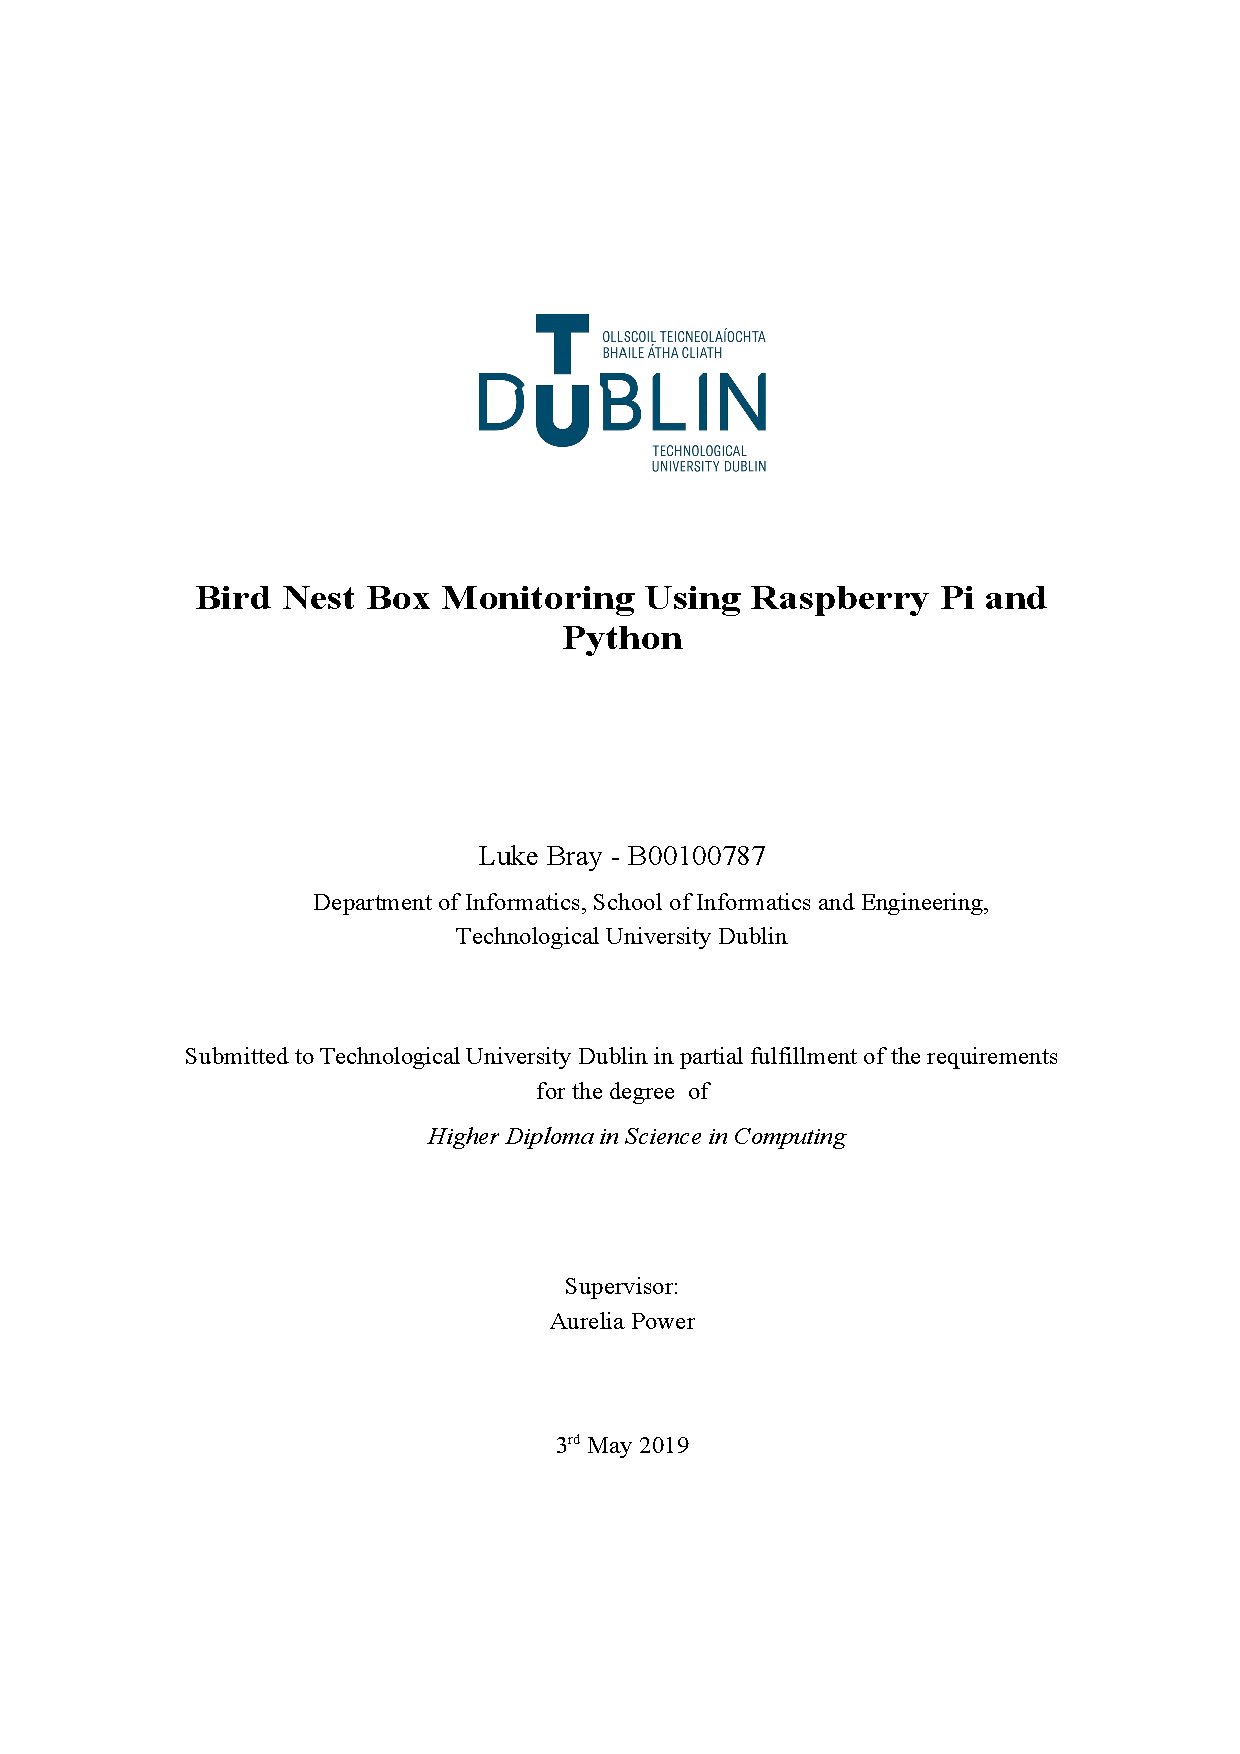
\includepdf[pages=-]{title_page.pdf}
\pagebreak
\section{Abstract}
\pagebreak
\section{Acknowledgements}
\pagebreak
\tableofcontents
\pagebreak
\listoffigures
\pagebreak
\listoftables
\pagebreak
\section{Introduction}
\subsection{Background}
Man-made nest boxes are vital for native cavity-nesting birds. One of the main reasons for this is the increased competition for natural cavity spaces. Non-native invasive species such as Starlings and House Sparrows as well as increased urban sprawl have reduced the number of available natural cavities. The Irish landscape is one that is heavily agricultural and changes in agricultural policies and practices have provoked losses in biological diversity\cite{PIERRET201814}. Therefore as the Irish landscape and policies governing it change it becomes ever more important to monitor the populations of all birds to see how they are faring\cite{website:birdwatchireland}. 

Monitoring a nest box is important for many reasons. First of all it can be interesting to see what kind of species is occupying the box. However this can be achieved by simply observing the coming and going of the box inhabitants. One of the biggest threats to nest boxes can be invasive species. This can include larger bird species and small mammals as well as insects and spiders. In this case it is helpful to have a view into the box. This can be achieved by physically inspecting the nest box however this can be intrusive and disturb the wildlife inside. Thus arises a need for a remote monitoring system using a non-intrusive camera. 

Maintaining a healthy habitat is important for the wildlife inside the nest box. Different species of bird are responsive to changes in environment at varying levels and some environmental factors can be critical to the survival of some species\cite{wormworth06}. It is for this reason that some simple monitoring equipment would be useful to include in any kind of nest box monitoring system.

All of the data that will be gathered is not very useful if it cannot be stored and displayed in a meaningful way. One of the most convenient ways to view data is through a graphical means and the particular data being collected in this project may be of interest to the public and anybody who has an interest in wildlife. Therefore it will be necessary to find a suitable way to store the data and display it in a way that is accessible and engaging. 

\subsection{Aims and Objectives}
From the background information provided above it becomes clear that there are definitely two main aims of this project. There will also be a third aim that is secondary to the function of the project however is equally important. 

The first aim of this project is to have an effective and useful monitoring system. This first aim can be broken down into multiple objectives. 
\begin{itemize}
\item To use appropriate hardware to capture the most important and fundamental data. In this context hardware refers to the actual computing device as well as the sensors that will be used to collect the data. Hardware that is used to power the device is also included in this objective as this will be important to ensure the completion of the objective.

\item To have efficient and appropriate software running on the hardware. The software is important as it is what controls how the data is processed, stored and displayed. It will have to be robust enough that it can handle large amounts of data and it should be designed in a way that allows the aim to be achieved. 

\item To design a system that is unobtrusive to the wildlife that will potentially inhabit or are currently inhabiting the nest box. If the device is too obtrusive then it is unlikely that birds will actually use it as a habitat and therefore no data can be collected. Similarly if the hardware and software are not well designed then regular maintenance will have to be performed which could lead to intruding on any wildlife that may be inhabiting the nest box and rendering the habitat useless. 
\end{itemize}

The second aim of this project is to display the collected data in a suitable way. This second aim can be broken down into multiple objectives.
\begin{itemize}
\item To display the sensor data in a graph or table that is easy to read and interpret. Historical data should also be available for analysis. 

\item To display the video footage captured by the camera. It is important that the footage is displayed live and if possible alongside the sensor data. 

\item To make the data easily available to anybody who would like to view it. This will mean hosting the data online. 

\item To capture the data without significant loss. The software will need to account for periods of time in case an internet connection cannot be obtained and it should be an objective to capture all data without significant loss. 
\end{itemize}

The third aim of this project is to enhance my learning and understanding of developing software and managing a project. This third aim can be broken down into multiple objectives. 
\begin{itemize}
\item To abide by a software development process and have thorough design documentation before any implementation is done. 

\item To have a proper software testing process in place that will minimise bugs and errors at implementation

\item To design a system that allows for future expansion in case I find that the project could be expanded. 
\end{itemize}

\pagebreak
\section{Literature Review}
\subsection{Introduction}
Birds have been used as tools all over the world for centuries for things such as hunting, entertainment and delivering messages. In the modern world bird watching is an already a popular activity and it's recent increase in popularity has helped to integrate research into birds, bird conservation and socio-economics development\cite{Zhijun2013}. In China alone as of 2010 there were in excess of 20,000 birdwatchers\cite{Zhijun2013}. The hobby is essentially the monitoring of different bird species and recording information such as the time of year, the species of the bird and how many birds there are. Many countries have organisations where birdwatchers can submit this data and this leads to an overall picture of the welfare of a countries native species.

A parallel to this rise in birdwatchers over recent years has been the emergence of the large number physical objects which are connected to the internet, commonly known as the \textit{Internet of Things}. These devices can play a large role in our daily lives and in 2010 the number of devices connected to the internet surpassed the population of humans on Earth\cite{AlFuqaha2015} and by 2020 it is estimated that the number of IoT smart objects deployed globally will reach 50 billion entities\cite{Arumuga2017}. 

When we see the clear trend upwards in both bird watching and smart devices connected to the IoT it becomes a natural step to combine the two and create a smart, connected device that can bring the hobby of bird watching and all of the benefits it provides into the digital world. Bird watching is essentially a hobby where monitoring takes place, albeit manually. It therefore seems natural with the help of small, powerful computers and all of the sensors available for them to build a monitoring device. 

In this literature review I will explore some other monitoring projects which used technology similar to that I intend to use. Creating a bird monitoring device will present some challenges such as connectivity and power supply and I will attempt to gain a better understanding of how I might cope with these challenges in my monitoring device.
\subsection{Raspberry Pi for Video Capture}
The main function of the device will be to capture a live video feed in the nest box to see what species of bird are nesting inside and some of their behaviours. One of the considerations to be taken when capturing video is how it will be transferred. Traditional monitoring camera systems such as Closed Circuit Television (CCTV) have poor video quality and rate of transfer. It is important for the device to be used for this paper to have high definition video with low latency times. One article\cite{Jennehag2016} set out to verify that high quality video could be transferred with low delay times using small, low-powered computers such as the Raspberry Pi. 

The aims of the study were to create a system that meets the following requirements:
\begin{itemize}
\item A low delay from source to sink of \textless200ms to provide an as close to live as possible viewing experience
\item High definition video content of at least 1280x720 at 25 frames per second
\item Runs on cheap, resource-constrained device such as Raspberry Pi
\end{itemize}

To achieve a stable transmission of video that does not saturate a network, video compression is usually required. One of the most popular video compression formats that is used is the H.264 and that is what is used in the article discussed here. Fortunately the Raspberry Pi camera modules (both IR and non-IR) were designed with high quality video streaming in mind and as such capture video as raw H.264 video stream\cite{piDoc}. The H.264 codec was created to provide good video quality at lower bit rates which makes it an ideal format for internet video streaming\cite{Wiegand2003}. The article discussed found that from source to sink, the average delay was 181ms at the specified resolution which met the requirements of their study.

One problem with the above study is that all of their tests were done using wired connection since the Raspberry Pi 2B that they used didn't have the ability to transmit via wireless connection. Given the remote nature of the monitoring system for this project the connection will most likely have to be wireless and I would expect that delay time will be greater than 181ms. However the study did find that 90\% of the total delay is due to the encoding and decoding of the video so I believe the increase in delay using a wireless transmission will be minimal. I am also happy that very low delay times are not a key requirement of this project.
\subsection{Raspberry Pi as Monitoring Device}
While live video feed is intended to be the main function of this device, the secondary function is to monitor the environment the device is placed in and measurements will be recorded by the device to achieve this. 

Many other papers have attempted to do this. One such paper, which was intended to create an IoT urban based climate monitoring system, found that due to its low cost and high reliability the Raspberry Pi was a good choice for a small, low powered monitoring system\cite{Shete2016}. The study used a Raspberry Pi 2 Model B along with 5 sensors to provide a broad overview of the surrounding environment. The system used Adafruit IO which provides different libraries that are used for implementing an IoT device. The libraries are available in many different languages however the one that was used here was Python. Adafruit IO can also generate a dashboard automatically containing graphs of the outputs from the various sensors which was useful to the study to display data in a meaningful, easy-to-understand way. 

One of the issues that the article discussed above did not address is how the device is powered. This is an important aspect of a monitoring device as they need to be constantly running to collect meaningful data.

Another study\cite{Sriyanka2017} used an Arduino board to house the sensing units which then transferred the data via Zigbee to the Raspberry Pi 3 which uploaded and processed the data onto the internet. The advantage of this is that the Arduino can be used as a separate sensing unit and the Pi can be used as the computing unit. This will increase performance across the two devices although it does add complications because the data has to be transferred to the Pi and then also to the internet. This wouldn't be a problem for a device that doesn't make use of Pi Camera module because the Pi can be safely located indoors however for this project the Raspberry Pi must be located close to the nest box so that the Pi Camera can be attached inside. 

Another problem with the above study is that it does not mention how the Arduino sensor module or Raspberry Pi are powered. They have stated that the system could potentially run for months without human intervention but have not discussed how the devices could be powered for this amount of time. This is something that I will try to discover in the next section.
\subsection{Powering the Raspberry Pi}
Raspberry Pi is powered by a +5.1V micro USB port and it is recommended to purchase a 2.5A power supply for stability reasons. According to the documentation a typical Raspberry Pi 3 Model B can use between 700-1000mA\cite{piDoc}. 

One paper set out to achieve an accurate estimation of the Raspberry Pi's power consumption and see if they could reduce power consumption by optimizing the software running on the platform\cite{Kaup2014}. In the study they set the Pi up to run only essential operations and specifically wrote lightweight utilization software to reduce power consumption while still achieving their goal. The monitor was not even permitted to write to the SD card, instead writing the results to RAM and copying the data after the monitoring had finished. The above was done with the intention of being able to monitor system utilisation without the process of monitoring affecting results. 

The study then used software called \textit{cpulimit} to generate load on the system. This software creates an infinite loop which adds numbers until the CPU load is at the desired limit. The study ended up with 900,000 power measurements which were combined and plotted logarithmic-ally in a heat map fashion on the graph below:

\begin{figure}[H]
\centering
  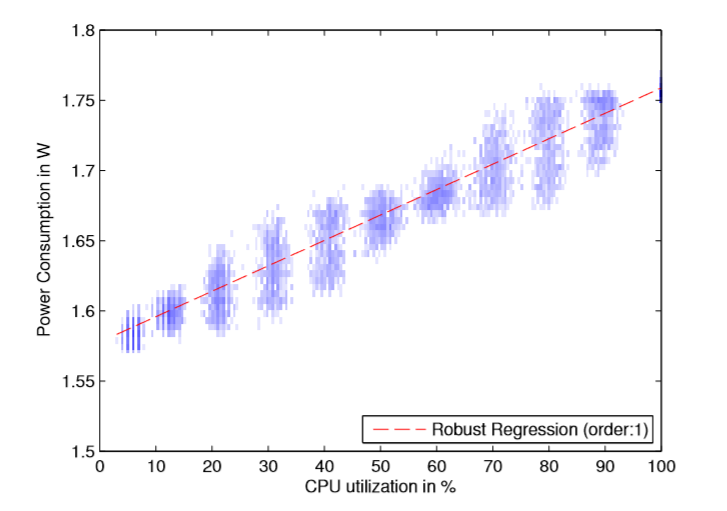
\includegraphics[width=\linewidth]{images/powerconsumption.png}
  \caption{Power consumption vs. CPU utilisation\cite{Kaup2014}}
  \label{fig:pwervscpu}
\end{figure}

The graph shows that CPU usage and power consumption have a linear relationship and as CPU usage reaches 100\% power consumption is at approximately 1.75W or 1750mA. This far exceeds what is stated in the documentation from Raspberry Pi although it can be argued that a Raspberry Pi will very rarely be close to 100\% CPU usage for any extended period of time. The study also attempted to model power consumption during network transmissions and found that using Ethernet consumed far less power. At 50MBit/s Ethernet had upload/download power consumption of ~0.3W and ~0.32W respectively. While WiFi used over 1.5W on both upload and download. 

The study above is a good example of how to measure the power consumption of a small device and could be easily adapted to measure devices other than the Raspberry Pi. It does highlight the need to think carefully about the types of transfer methods used as these can clearly have a significant impact on power consumption.
\subsubsection{Solar Power}
It seems that the most efficient way to power a monitoring system would be to use a renewable energy source. The most accessible and affordable is solar power. A solar power system has three main components: 
\begin{enumerate}
\item\textit{The Solar Panel} - This is what most people think of when they think of solar power. It is a panel that uses the photo-voltaic effect to convert sunlight and to electricity and is the core of any solar power system.
\item\textit{The Solar Controller} - This is an important part of any solar power system. It's role is to regulate the amount of charge coming from the panel to the battery and prevent overcharging\cite{website:energymatters}. Devices can also be charged directly from the solar controller with some versions even including 2.5A USB ports which are ideal for charging devices such as Raspberry Pi.
\item\textit{The Battery} - This part of the solar power system is optional. If you have a device which is being charged directly then there will be no need for this part of the system however it could be important in climates where there is not a lot of sunlight or if you have a device that needs to be powered overnight.
\end{enumerate}

With the three components above a typical solar power system circuit diagram might look like the one below: 

\begin{figure}[H]
\centering
  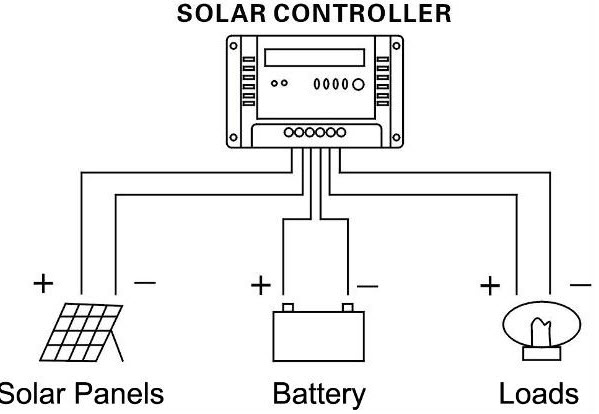
\includegraphics[width=\linewidth]{images/solarcircuit.jpg}
  \caption{A basic solar circuit\cite{website:edgefx}}
  \label{fig:solarcircuit}
\end{figure}

\subsection{Raspberry Pi Connectivity}
There are multiple options available for connectivity to the Raspberry Pi and 3 of the main methods will be explored below.
\subsubsection{WiFi} 
The latest model of the Raspberry Pi comes with a built in 2.4GHz 802.11n wireless adaptor, allowing it to transmit data without any need to external adaptors or wires. There are many WiFi standards available however the most prominent is 802.11n and it is found in most wireless devices such as smart-phones, tablets and laptops. There is a competitor called 802.11ac which was developed to handle larger files and faster speeds. Several studies, including one by Ruckuswireless\cite{Ruckus2014}, have found that 802.11ac is a superior connectivity standard to 802.11n however the low cost of 802.11n has meant it has become the favoured standard and this is why it appears in the Raspberry Pi. 

802.11n can transfer data with throughput up to 300Mbps and over distances of 70 metres in open structure environment and 250 metres in open air environment\cite{Kaewkiriya2017}. This makes it ideal for transfer of relatively small amounts of data from a monitoring station however power consumption and reliability of WiFi in general still remain a cause for concern. WiFi also has quite weak security and the size of a WiFi network must remain relatively small with a maximum of around 16 devices on any normal network.  
\subsubsection{Wired Transfer}
Raspberry Pi 3 Model B comes with 1 Gigabit Ethernet over USB2.0 port. The use of USB2.0 means that the throughput is limited to 300MBps - the same as WiFi. We have already seen in\cite{Kaup2014} that Ethernet connections use significantly less power than WiFi however because the transfer is via USB2.0 we do not see the speed advantages that Ethernet connections generally offer. We will still get a faster connection because there will be no loss as there is with WiFi and using a wired connection means we get more stable speeds. Wired Ethernet connections are also more reliable that WiFi connections due to the removal of any chance of network interference from other transmissions.
\subsubsection{Zigbee Wireless Protocol}
Zigbee is wireless specification based on IEEE 802.15.4 that was first seen in 2007 and is widely used in wireless monitoring devices due to it's low-cost and low-power requirements. This protocol describes only the MAC and physical layers\cite{Elarabi2015}. Zigbee uses small, low-powered and low-cost radios to transmit signal. The data transfer rate of Zigbee is 250Kbits/sec. It can operate on 2 regional frequency bands (868MHz in Europe, 915MHz in America) and 1 global 2.4GHz frequency band\cite{ZigbeeAlliance}. 

A strength of Zigbee is that it can transmit signal at distances of up to 100m between sender and receiver. One criticism has been that their needs to be line of site between sender and receiver however there have been papers that suggest signal strength may not be affected by obstacles. Idoudi, 2013 used the Received Signal Strength Indicator (RSSI) to show that there was little other than distance between two nodes that negatively affected RSSI values and that distance had a more negative effect on RSSI than any obstacles in the way\cite{Idoudi2013}. However the study did not state the distance between two nodes when the obstacles were placed between them. RSSI indicates the strength of the signal at the receiving node. 

Interference with Zigbee from WiFi can also occur and this is one of the main drawbacks of Zigbee, along with the rate of transfer. Zigbee uses 16 channels within the 2.4GHz band and these directly overlap with the 3 channels used by WiFi. This is shown in the figures below:

\begin{figure}[H]
\centering
  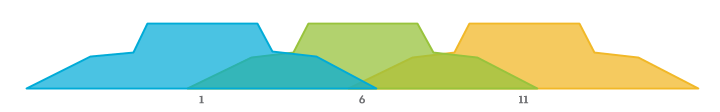
\includegraphics[width=\linewidth]{images/wifi_channels.png}
  \caption{2.4GHz WiFi Channels\cite{zigbeechannels}}
  \label{fig:wifichannels}
\end{figure}

\begin{figure}[H]
\centering
  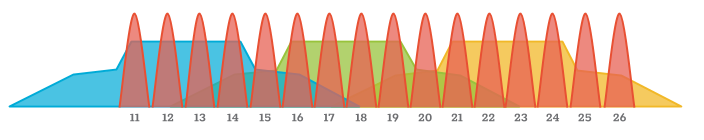
\includegraphics[width=\linewidth]{images/zigbee_channels.png}
  \caption{2.4GHz Zigbee Channels\cite{zigbeechannels}}
  \label{fig:zigbeechannels}
\end{figure}

Usually the Zigbee network is the network that will lose packets. The side band lobes of the WiFi signal can easily drown out the less powerful Zigbee signals. This is one of the biggest problems with Zigbee and careful planning is required when it will be used in close proximity with any WiFi-enabled devices.

\subsection{Python Web Frameworks}
A key aspect of this project is to display the collected data in a way that is appealing and accessible. This will most likely mean displaying the data on a web page. However due to the rapid evolution of the World Wide Web it has become difficult to utilise all of the technologies required for good web development\cite{pop_altar_2014}. Using a web framework can be a good way to tie the various technologies together to allow for quicker development and also to facilitate future expansion more easily. This section will look at three Python web frameworks and discuss some of their features. 
\subsubsection{Django}
Django\cite{website:django} is a free, open-source Python web framework. It is a Model View Controller (MVC) style framework and is focused on never having to repeat yourself when programming. Django is a framework that allows for quick development and minimal repetition of code. It also ensures that your app is secure against a multitude of vulnerabilities. This richness of features is also one of the main criticisms against Django. While the vast array of features may be ideal for a large scale project, they are not needed for a smaller scale project. Django is also considered to be quite monolithic and not hugely flexible. You get features such as admin panels and database interfaces out of the box which means it is not nearly as customisable as some other frameworks. 
\subsubsection{Flask}
Flask\cite{website:flask} is seen by many to be the main rival to Django. Like Django, it is a MVC style framework however it is not nearly as feature-rich and provides only the more essential features. This more minimalist design means that Flask may be better suited to smaller project however there are some large projects such as Netflix and Pinterest which are built on Flask. This may be an indicator that there is also good scalability with Flask. 
\subsubsection{Dash}
Dash\cite{website:dash} is a micro-framework that is built on top of Flask and Plotly.js. The framework includes various UI elements and allows you to tie them together with Python code while also retaining all of the benefits of using a MVC framework like Flask. Dash is specially built to be used for building analytical web applications and this makes it ideal for a project where data is to be presented and analysed. 

\pagebreak
\section{System Requirements and Design}
\subsection{Introduction}
This chapter will outline the key requirements of this project and will then identify how the key software components interact with each other to meet these requirements. Requirements will mainly be derived from use cases and these will be important in identifying any previously unforeseen issues that may arise. UML diagrams will demonstrate the context and modes of use of the system as well as the system architecture, primary system objects, design models and specific interfacing methods. 

\subsection{Use Cases}
\subsubsection{Stream a Live Video Feed}
\begin{table}[h!]
\centering
\begin{tabular}{p{2cm}p{9cm}}
\toprule
\textbf{Use Case}    & Stream live video feed                                                                          \\ \midrule
\textbf{Actors}      & PiCamera, Raspberry Pi                                                                          \\
\textbf{Description} & The PiCamera sends live video over the internet to YouTube while the device is running         \\
\textbf{Stimulus}    & Started via command in command line                                                             \\
\textbf{Response}    & Video data is captured according to settings in command and is streamed to Youtube              \\
\textbf{Comments}    & The streaming of video data will rely on a constant internet connection as well as power supply \\ \bottomrule
\end{tabular}
\caption{Use Case 1 - Stream a live video feed}
\label{tab:useCase1}
\end{table}

\subsubsection{Record Environmental Data}
\begin{table}[h!]
\centering
\begin{tabular}{p{2cm}p{9cm}}
\toprule
\textbf{Use Case}    & Record environmental data                                                                          \\ \midrule
\textbf{Actors}      & Data sensors, Raspberry Pi, web server                                                                          \\
\textbf{Description} & The various sensors will record data about the environment including if it is raining or not, temperature and humidity. The data will be sent to a web server         \\
\textbf{Stimulus}    & Triggered by software application\\
\textbf{Response}    & Data is captured and sent to the web server              \\
\textbf{Comments}    & The streaming of data will rely on a constant internet connection as well as power supply \\ \bottomrule
\end{tabular}
\caption{Use Case 2 - Record environmental data}
\label{tab:useCase1}
\end{table}

\subsubsection{Display Environmental Data}
\begin{table}[h!]
\centering
\begin{tabular}{p{2cm}p{9cm}}
\toprule
\textbf{Use Case}    & Display environmental data on a web page \\ \midrule
\textbf{Actors}      & Data sensors, PiCamera, Raspberry Pi, web server, web page, web user                                                                          \\
\textbf{Description} & The website will make a request to the web server to grab the data and the data will then be output to the web page in a way that is visually appealing         \\
\textbf{Stimulus}    & Triggered by user accessing the web page\\
\textbf{Response}    & Data is retrieved from the web server and displayed on the web page              \\
\textbf{Comments}    & The streaming of data will rely on a constant internet connection and the web server to remain connected \\ \bottomrule
\end{tabular}
\caption{Use Case 3 - Display environmental data}
\label{tab:useCase3}
\end{table}

\begin{figure}[H]
\centering
  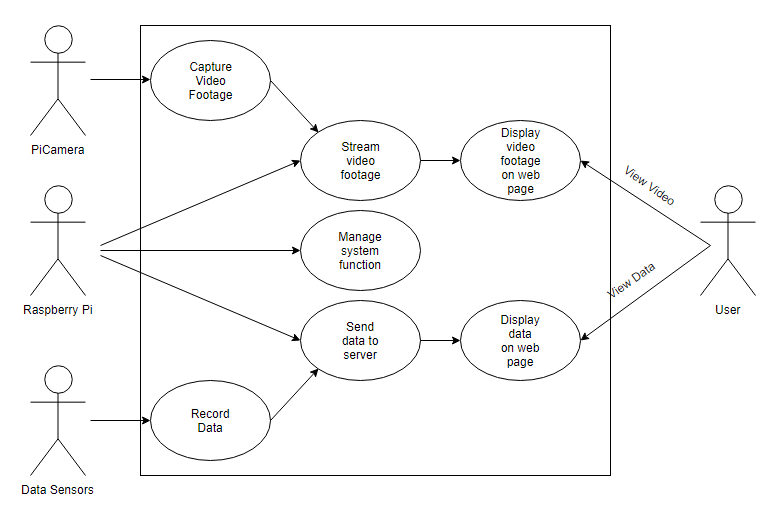
\includegraphics[width=\linewidth]{images/use_case_diagram.png}
  \caption{Use Case Diagram}
  \label{fig:usecasediagram}
\end{figure}

\subsection{System Requirements}
\subsubsection{PiBB - SR001}
The system will be able to output a live HD video feed of the inside of the dark nest box. This allows a user to see if anything is living inside of the nest box.
\subsubsection{PiBB - SR002}
The system will be able to record environmental data about the nest box and send it to a web server.
\subsubsection{PiBB - SR003}
The web server must be able to display live data and the web page must update dynamically to display the latest data
\subsubsection{PiBB - SR004}
The system will be able to interpret the data received from the sensors and display live data on a dynamic web page. This allows a user to see environmental data.
\subsubsection{PiBB - SR005}
The system will be able to be deployed remotely and outside. This will mean having a renewable power source and wireless internet connection. The system must be weatherproof.
\subsubsection{PiBB - SR006}
The system will be able to manage power failures in a way that does not corrupt or damage files on the system
\subsubsection{PiBB - SR007}
The system must not be obtrusive to the wildlife occupying the nest box and must be as discreet as possible. 
\subsubsection{PiBB - SR008}
It must be possible to access the system remotely to perform necessary software maintenance once it is deployed. 
\subsubsection{PiBB - SR009}
The sensor and camera controllers must be built using Python programming language.
\subsubsection{PiBB - SR010}
The web application should be built using a Python framework.
\subsection{Power Supply}
For a remote monitoring device the power supply is one of the most crucial aspects of the design. The power supply has to provide enough power for the device to be continuously powered but it also needs to be renewable. Below I have explored the option of using solar power.
Solar power has been chosen because it is a renewable energy source therefore being environmentally friendly. It is also the most accessible renewable energy source in that to generate solar power is quite cheap and efficient despite the fact that we do not live in a particularly sunny country. Having solar power also removes the need for an electricity supply and this makes the device more portable and increases the versatility. 

Power consumption of the Raspberry Pi with various configurations is shown in the below table. 

\begin{table}
  \centering
  \resizebox{\linewidth}{!}{%
  \begin{tabular}{lllllllll}
  \textbf{Configuration} & \textbf{Volts} & \textbf{Amps} & \textbf{Watts} & \textbf{Watts(+15\%)} & \textbf{24H Req.} & \textbf{18HR Req.} & \textbf{12HR Req.} & \textbf{6HR Req.} \\
  Raspi & 5.06 & 0.4 & 2.0 & 2.3 & 56 & 42 & 28 & 14 \\
  Pi + Sensors & 5.06 & 0.4 & 2.1 & 2.4 & 58 & 43 & 29 & 14 \\
  Pi + Camera + Sensors & 5.09 & 1.3 & 6.6 & 7.6 & 183 & 137 & 91 & 46
  \end{tabular}}
  \caption{Monitoring system power requirements}
  \label{tab:powerRequirements}
  \end{table}

As can be seen from the table above, to run the system for 24 hours would require 183W of power. However running the system for 18 hours per day only requires 137W. With a 60W solar panel this could be achieved with 3 hours of sunlight per day. 

As the device will be located in Ireland it is important to have an understanding of the sunshine levels. Ireland gets, on average, 1100-1600 hours of sunshine per year\cite{website:metsunshine}. This translates to roughly 5-6.5 hours in the Summer months and 1-1.5 hours in the Winter months. This means that in the Summer months the device may be able to run for up to 18 hours per day however to be conservative it would be safe to say that during the summer months the device could run for 12 hours per day. Cloud cover is not as predictable of sunshine hours and so the actual amount of sunlight the panel receives may be less than anticipated. In this case the device will have to run for less time during the day or a larger solar panel will have to be installed. 

There is one problem with using solar power. The Raspberry Pi cannot be put into a sleep mode - it is either on or off and there is no low power mode. If the device is shut down while it is writing to the SD card there is a danger that the operating system could be corrupted. This would be problematic if there was no available sunlight or the backup battery ran out. Due to the fact there is no sleep mode it also means the Pi cannot be powered on and off strategically and remotely which renders the device useless as a remote monitoring device. 

Products and modifications are available that allow the Pi to go into a power saving mode however these are expensive and beyond the scope of this project. For this reason, for the purposes of this project, the device will be powered via USB plugged into an outlet. The device will still have use as a monitoring system in a garden. Use of alternative renewable energies such as wind power could be explored in a future iteration of the project.


\subsection{Connectivity}
A key requirement of this device is that it is able to function as a remote monitoring device. While Ethernet may be the most reliable form of connection, it is not the most portable as the range is limited by the length of cable you have. 

Another method that was discussed was Zigbee wireless transfer. However this method of transfer is very slow at approximately 250Kbit/sec. This would be good enough for data transfer to an external server but not video streaming. The range of Zigbee is also only 300m and this requires line of site meaning location of the remote device will be limited. 

This leaves WiFi to transfer the data. The device will connect to a 4G hotspot allowing it to use WiFi to stream video and send data to a web server. The provider will be Three who allow unlimited data and the portable hotspot will be powered by a battery pack at first with the option being powered by the solar system later on if it is efficient enough when implemented. 

\subsection{PiCamera}
To satisfy the requirement of capturing video footage from inside a dark nestbox the camera must be able to see in the dark. This can be achieved using a camera without an infra-red (IR) filter however there must also be an IR-emitting source for the camera to pick up. This device will use a specially modified PiCamera which will have no IR filter. Attached to the camera will be two IR-emitting bulbs and this will bathe the inside of the nest box in IR light which the camera can then pick up. 

The actual video footage can be streamed using a package from Libav called avconv. Avconv is a very fast audio and video converter which can process raw audio and video frames, convert them to the specified format and then encode and output them to a video streaming platform\cite{avconv}

\subsection{Web Framework and Data Display Web Page}
The web framework that will be used is called Flask. Flask is a more minimal Python web framework than Django and this means that it is more configurable and easier to set up. Flask uses SQLAlchemy which is the Python toolkit for working with SQL databases and this will make it easier to work with the large amounts of data this project will eventually accumulate. Flask makes use of Jinja2 which is a HTML templating language specifically made for use with Python. The use of this templating language should make creating the web page front end a lot simpler.

The web page will be a minimal single page displaying only an embedded video of the live stream and some chart components. The chart components will be created using the charts.js library and the live video will be hosted on YouTube and embedded into the site. Below is a sample wireframe of the web page. 

\begin{figure}[H]
\centering
  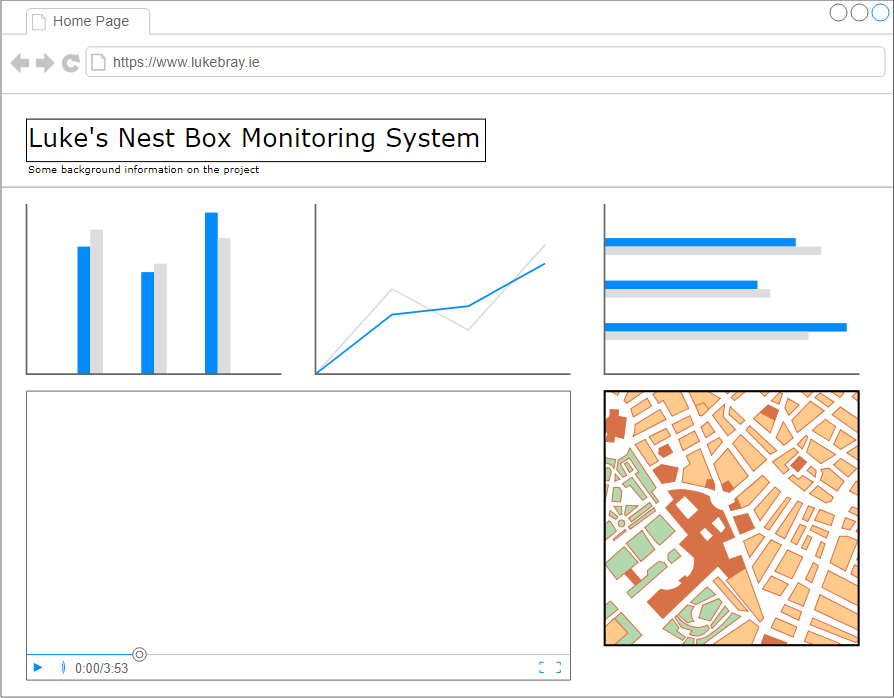
\includegraphics[width=\linewidth]{images/web_page_mock_up.png}
  \caption{Web Page Wireframe}
  \label{fig:webwireframe}
\end{figure}

\subsection{Object Classes}
The object classes presented in the diagram below are based on the hardware objects and data objects in the system as well as the controlling objects such as the Raspberry Pi itself. A summary of each object is presented below:
\begin{itemize}
\item DHT11 Sensor \& Rain Sensor - The hardware objects that are responsible for the data gathered in the system
\item PiCamera - This hardware object is responsible for capturing video data of the inside of the nest box
\item Raspberry Pi - The device which controls the system and is responsible for performing actual transmission of data. It's main function is to be a vehicle for management of the hardware components
\item Environmental Data - This object summarises the data gathered from the hardware instruments
\item Web App - This object is responsible for displaying data to the user 
\end{itemize}

\begin{figure}[H]
\centering
  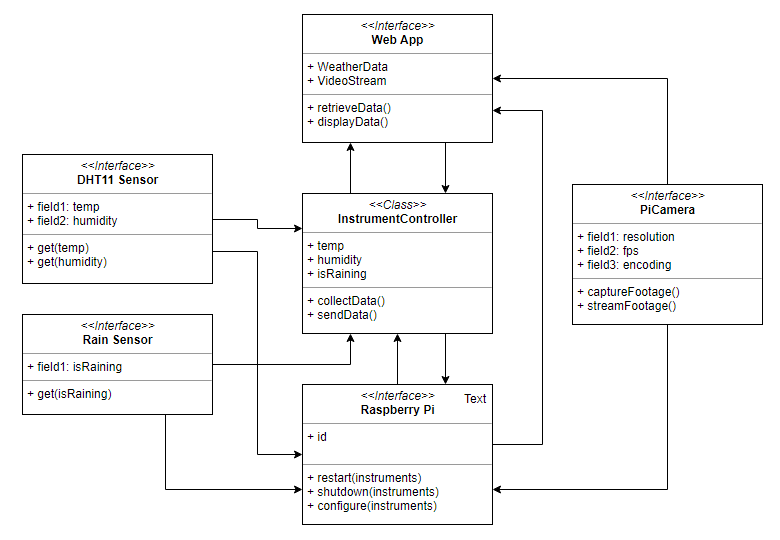
\includegraphics[width=\linewidth]{images/objects.png}
  \caption{Object Diagram}
  \label{fig:objects}
\end{figure}

\subsection{Development Environment Setup}
\subsubsection{Raspberry Pi}
The operating system used on the Raspberry Pi is called Raspbian OS (version 9). Raspbian is a debian-based operating system and is officially provided by the Raspberry Pi Foundation meaning it is the most compatible to run on a Raspberry Pi. I expect that using Raspbian will limit any potential issues. 

The installation process is very simple. I have downloaded NOOBS (New Out Of the Box Software) and copied the downloaded files to a newly formatted 16GB SD card. Then when booting the Raspberry Pi I selected Raspbian and the OS was installed without issue. 

Raspbian comes loaded with a Python 3 development environment which includes an installation of Python 3 and a Python IDE (Thonny). The development of data handling software will be done in this environment. 

The Raspberry Pi had to be configured to set up the VNC server. This can be done by opening a terminal and typing \begin{verbatim}
sudo raspi-config
\end{verbatim} From here the VNC server is enabled by selecting Interfacing Options \textgreater VNC and enabling the server.

\begin{figure}[H]
\centering
  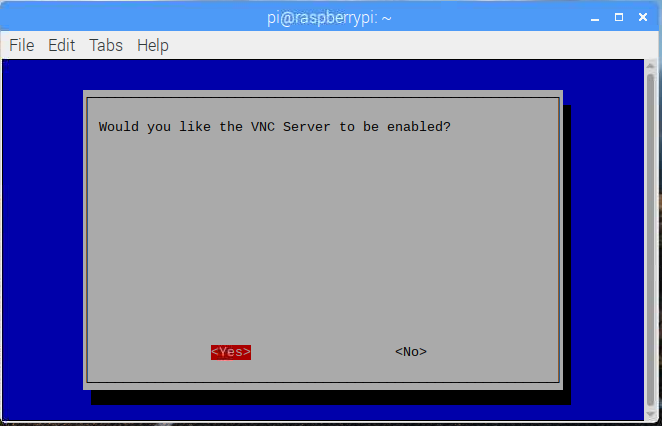
\includegraphics[width=\linewidth]{images/vncserver.png}
  \caption{Enabling VNC Server}
  \label{fig:vncserver}
\end{figure}

A similar process has to be performed for the Rasperry Pi Camera. This leaves the Raspberry Pi configured and after updating it is ready to use for development.

\begin{figure}[H]
\centering
  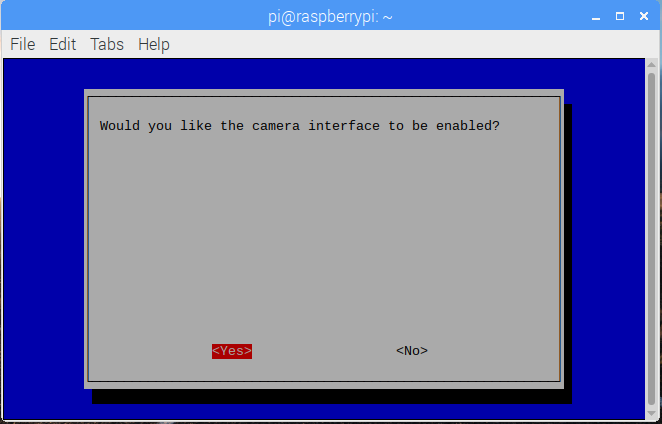
\includegraphics[width=\linewidth]{images/picamera.png}
  \caption{Enabling PiCamera}
  \label{fig:picamera}
\end{figure}

\subsubsection{Web Development Environment}
This project will use a web development environment called Python Anywhere. This is a web environment that allows access to the project from any web browser. Python Anywhere allows for easy creation of web apps using the most popular Python web frameworks and also allows for easy SQL database creation as well as providing the ability to run multiple consoles. There are security features built into Python Anywhere and it makes it very easy to obtain things such as HTTPS certificates. The versatility of Python Anywhere is the main reason I have decided to use it and not having to set up a Python environment on multiple machines is hugely beneficial. Also all of the code and databases are in the cloud which, when combined with version control such as Git, means that the project will be safer from any potential data loss.

Setup of a new web app is as easy as selecting the Framework you'd like to use and the version of Python to use.

\begin{figure}[H]
\centering
  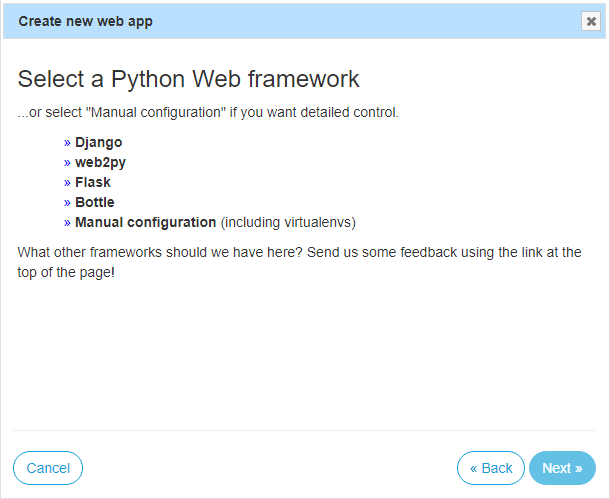
\includegraphics[width=\linewidth]{images/webappframework.png}
  \caption{Selecting a web framework on Python Anywhere}
  \label{fig:webappframework}
\end{figure}

\begin{figure}[H]
\centering
  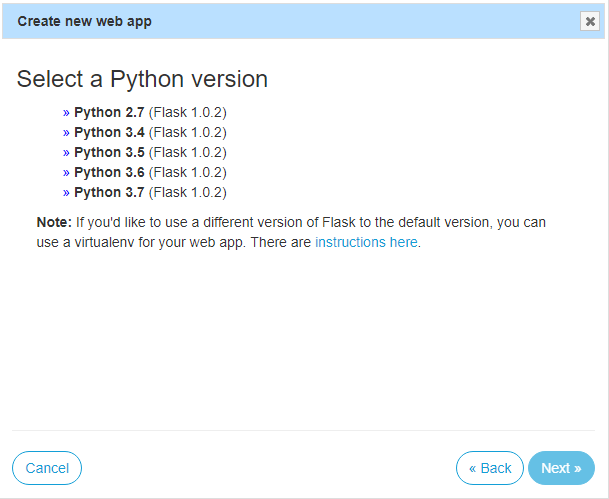
\includegraphics[width=\linewidth]{images/webapppython.png}
  \caption{Selecting a which version of Python to use}
  \label{fig:webapppython}
\end{figure}

Actual development of code will be done on my local machine using VSCode. The whole project will be stored in a Git repository which can then be cloned into Python Anywhere using one the virtual consoles. 

\pagebreak
\section{Implementation} 
\subsection{Introduction}
This chapter will cover how the software has been developed and how it is used within the project. It will aim to layout the different technologies that have been used, how they have been implemented and finally how they all work together to achieve the system requirements set out earlier in this document.

\subsection{Implementation Method}
Even in the early days of software engineering the criticality of having a sound software development approach was recognised. It can be easy to delay or avoid completing this process while deficiencies in it can be very difficult and expensive to correct later on. Other issues arise such as the user feeling alienated due to lack of transparency or documentation and testing being hard to define\cite{1674590}.

This project will be implanted using an iterative software development life-cycle. This type of methodology involves a planning stage where the requirements of the system are defined. The iterative part of the life-cycle see's the project designed, implemented, tested and then evaluated. This is important because the project can be split into multiple mini-projects that don't present as big of a task. This particular project has been designed to be modular and using an iteration development method allows each modular component to be thoroughly tested and integrated seamlessly into the overall project. Through testing it is ensured that every component of the design can work independently and then combine at a later stage to form one overall project. Each iteration of the project adds in a new component which brings with it extra features and stability. 

Each component of the project will be developed individually and then tested to make sure it works before introducing it into the final project. This is the advantage of using an iterative software development life cycle. A diagram of the life-cycle is shown below. 

\begin{figure}[H]
  \centering
    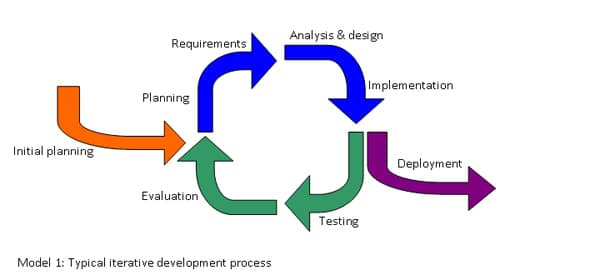
\includegraphics[width=\linewidth]{images/iterativemodel.jpg}
    \caption{Diagram of an Iterative SDLC}
    \label{fig:iterativemodel}
\end{figure}

\subsection{System Overview}
The physical prototype was built and is explained later in this chapter. A bash script has been written so that on startup a Linux command is automatically executed and this begins the streaming of the PiCamera to Youtube. The same bash script will also run dataSend.py. which uses classes dht11.py and rainSensor.py to record data. The data is then inserted into the MySQL database where it can be displayed on a web page. The Flask app processes the data and passes it to main.html and using the charts.js library the data is then displayed in a presentable manner. Main.html also embeds the live stream from Youtube. 

\subsection{Physical Environment Setup}
The first step of implementation was to get the hardware circuit working. The four main components are the Raspberry Pi, a DHT11 temperature and humidity sensor, the NoIR PiCamera and an FC-37 rain sensor. Initially these were implemented into a circuit using a breadboard. This allowed for a less permanent and more flexible setup for testing purposes. The circuit diagram is shown below along with some photographs of the hardware setup. 

\begin{figure}[H]
  \centering
    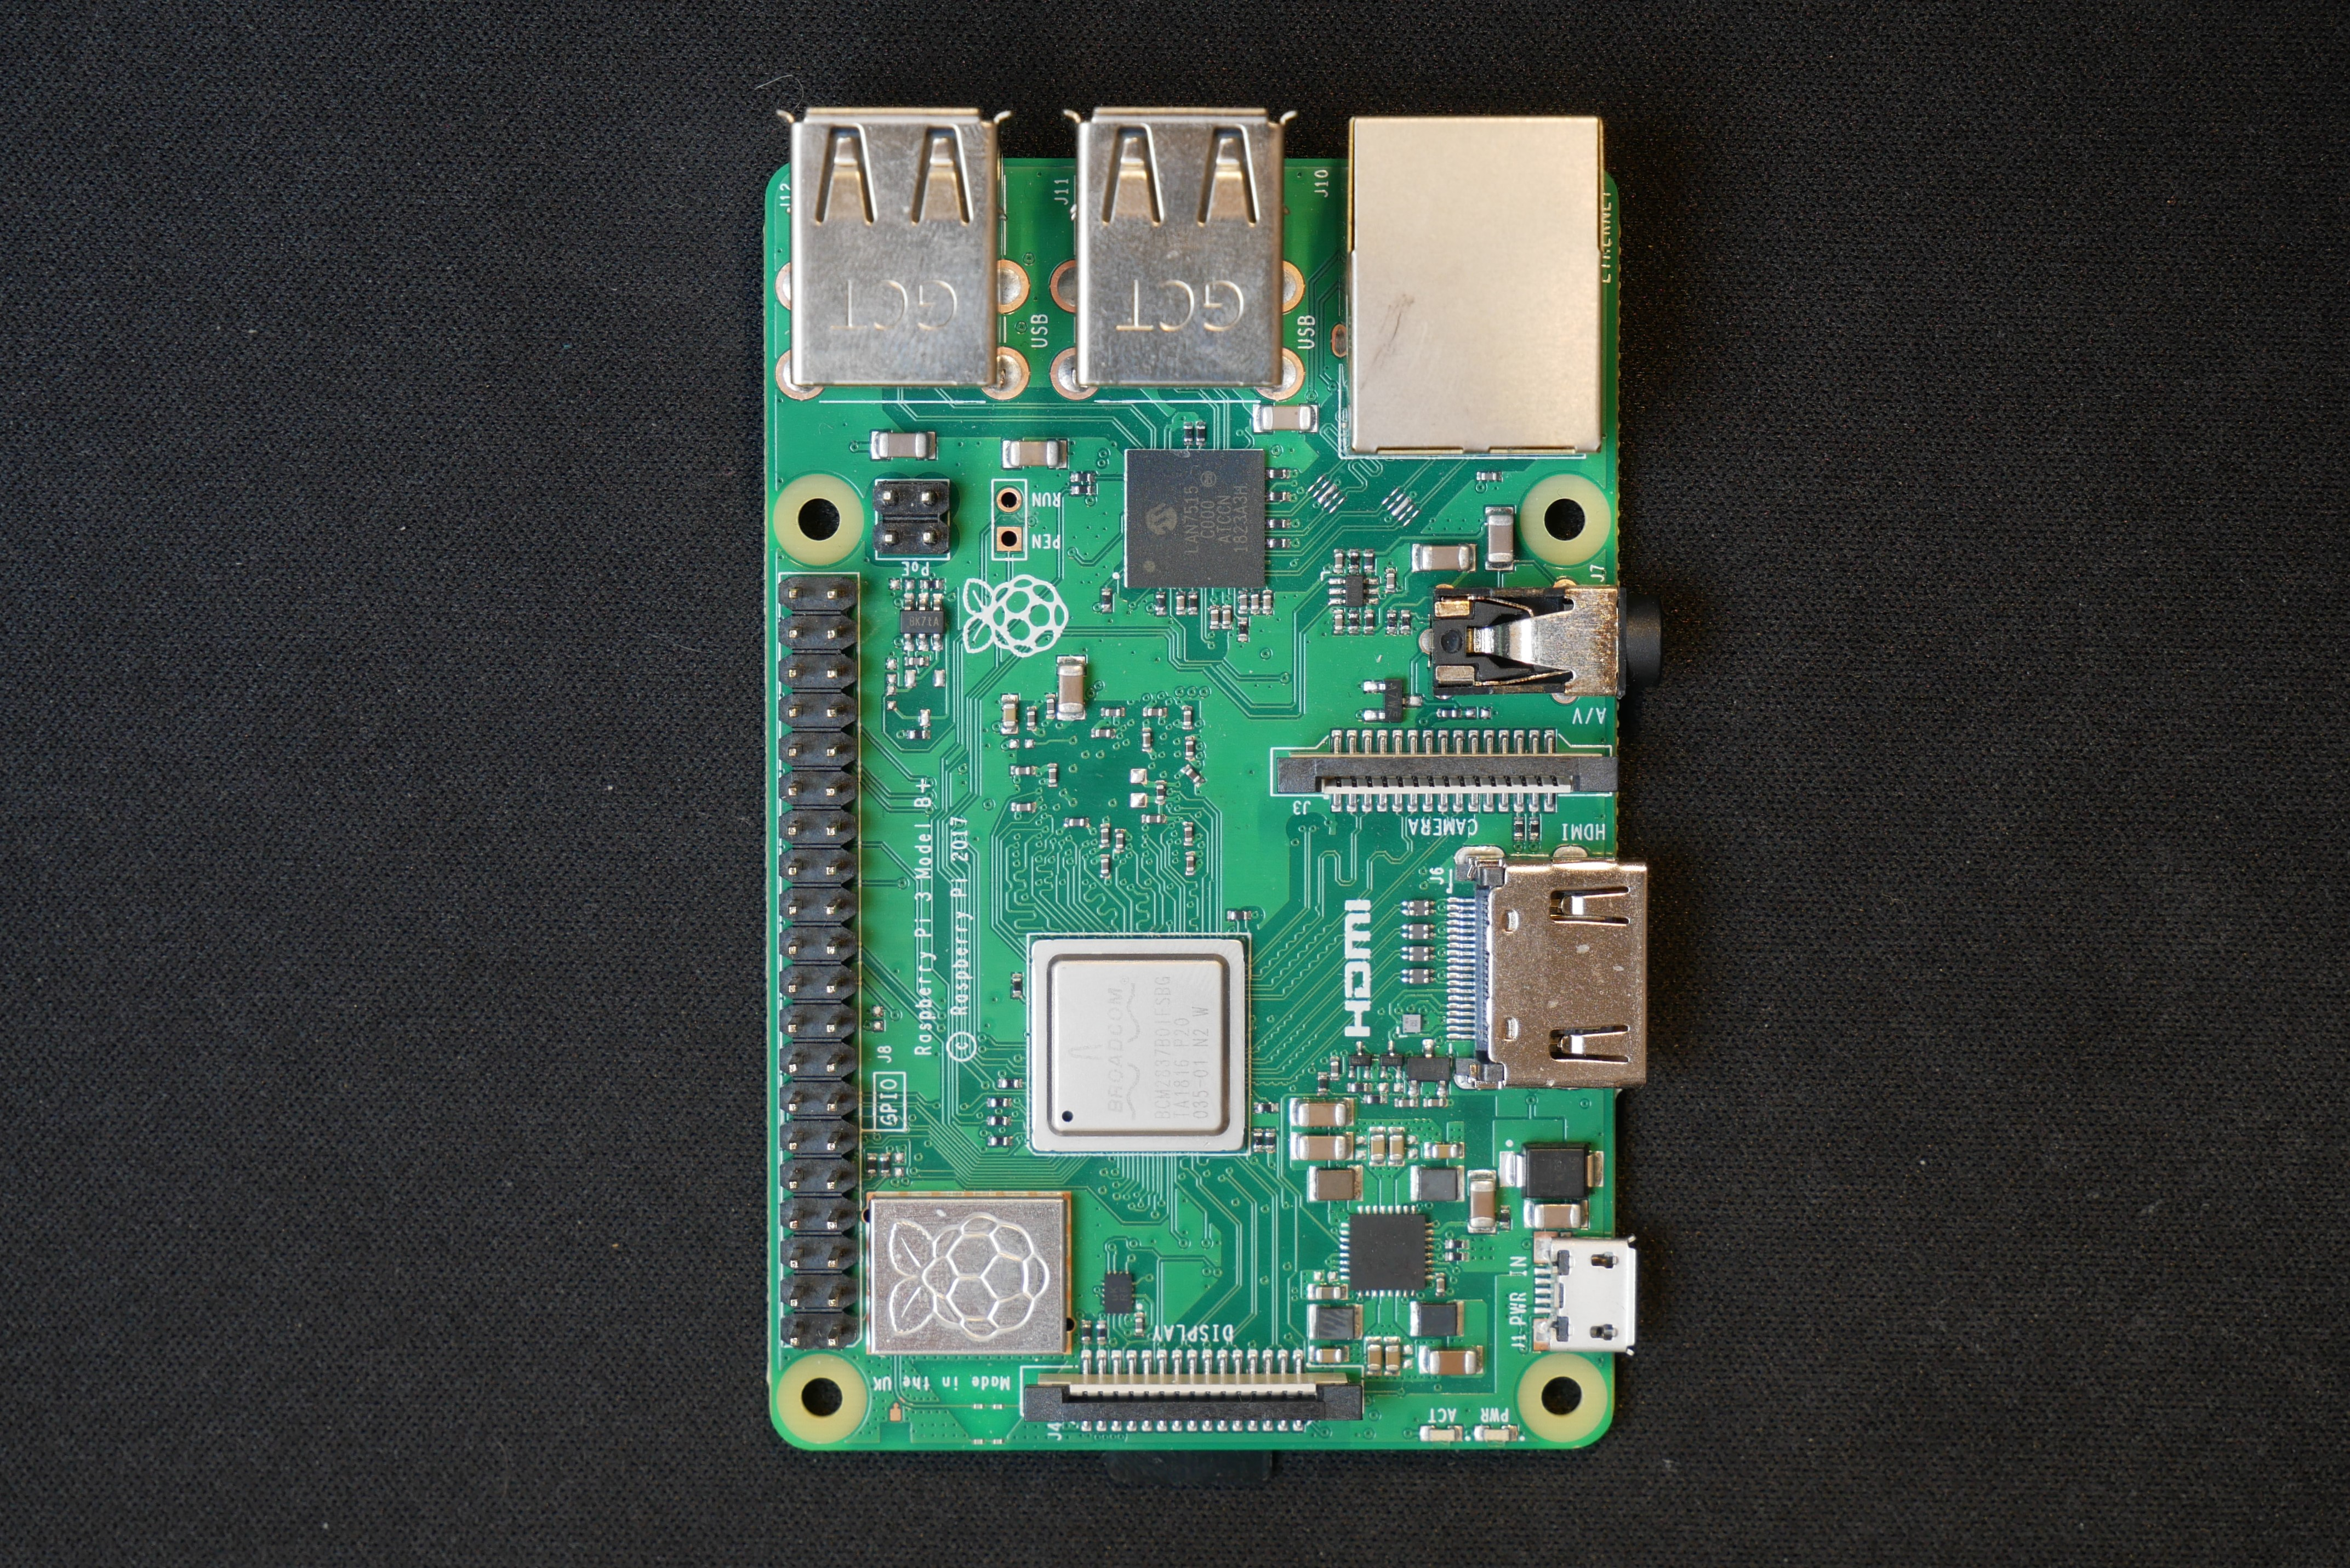
\includegraphics[width=\linewidth]{images/RPi.jpg}
    \caption{The Raspberry Pi}
    \label{fig:Raspberry Pi}
\end{figure}

\begin{figure}[H]
  \centering
    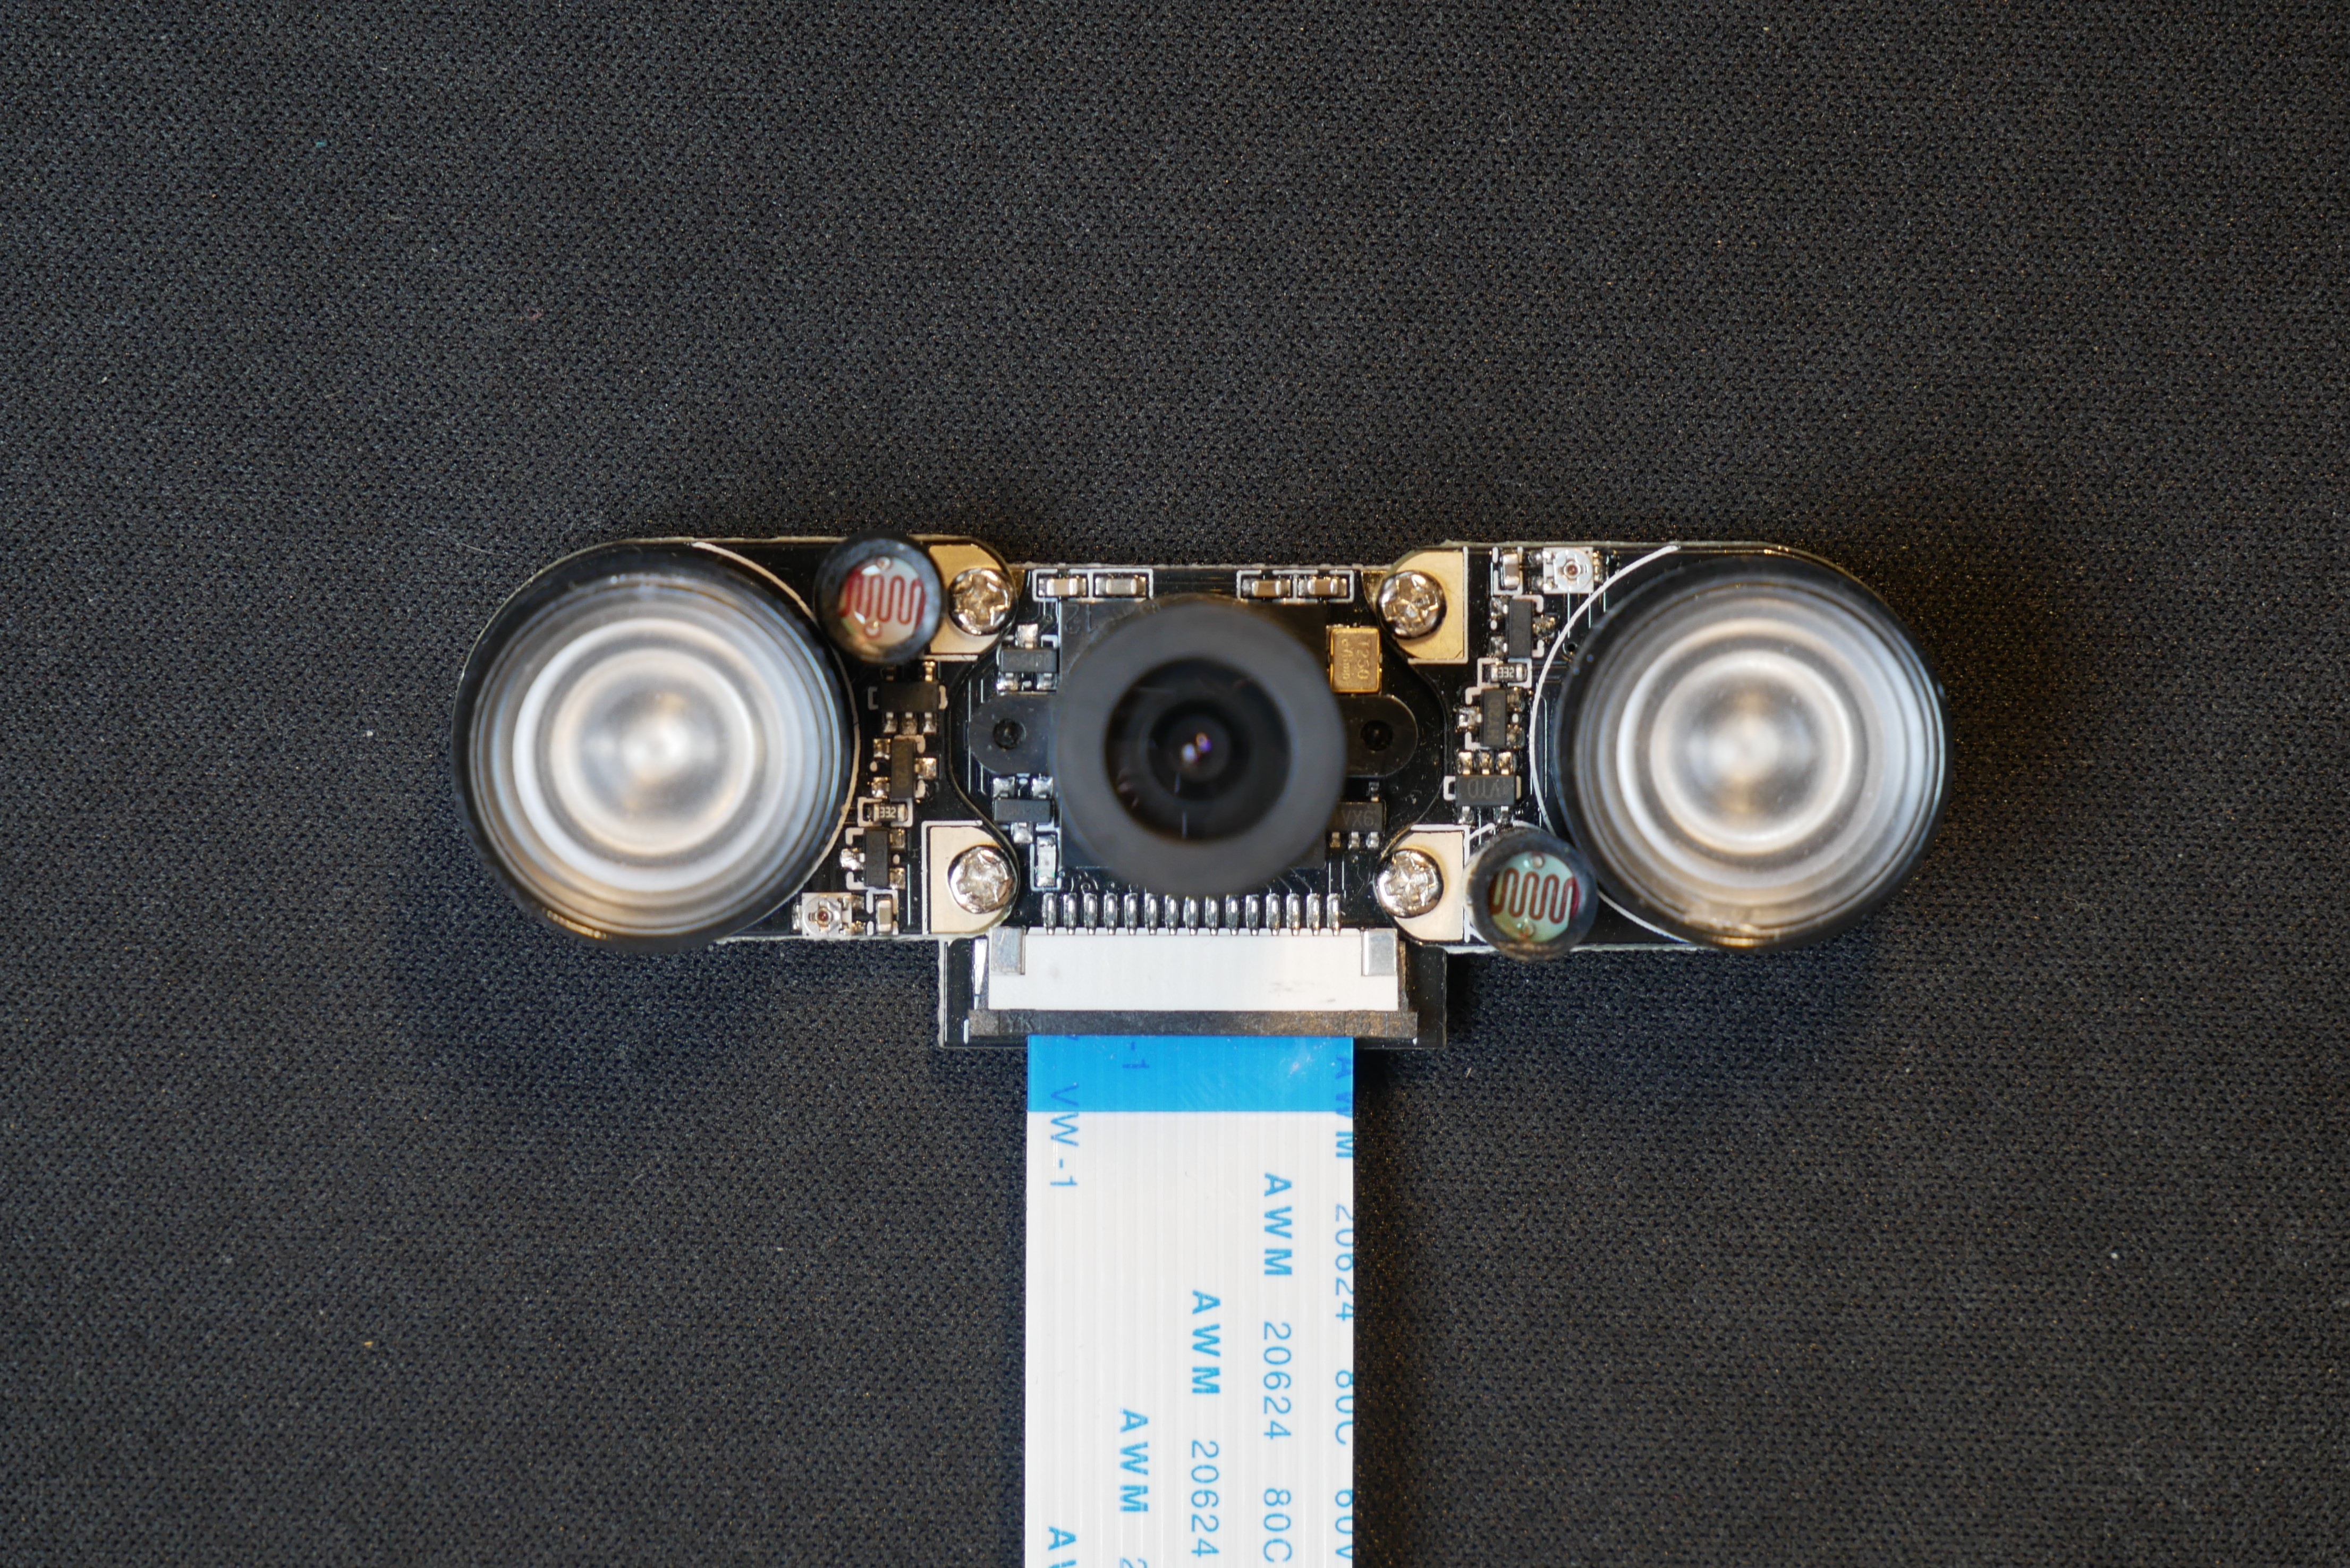
\includegraphics[width=\linewidth]{images/piCam.jpg}
    \caption{The PiCamera with IR bulb attachments}
    \label{fig:piCam}
\end{figure}

\begin{figure}[H]
  \centering
    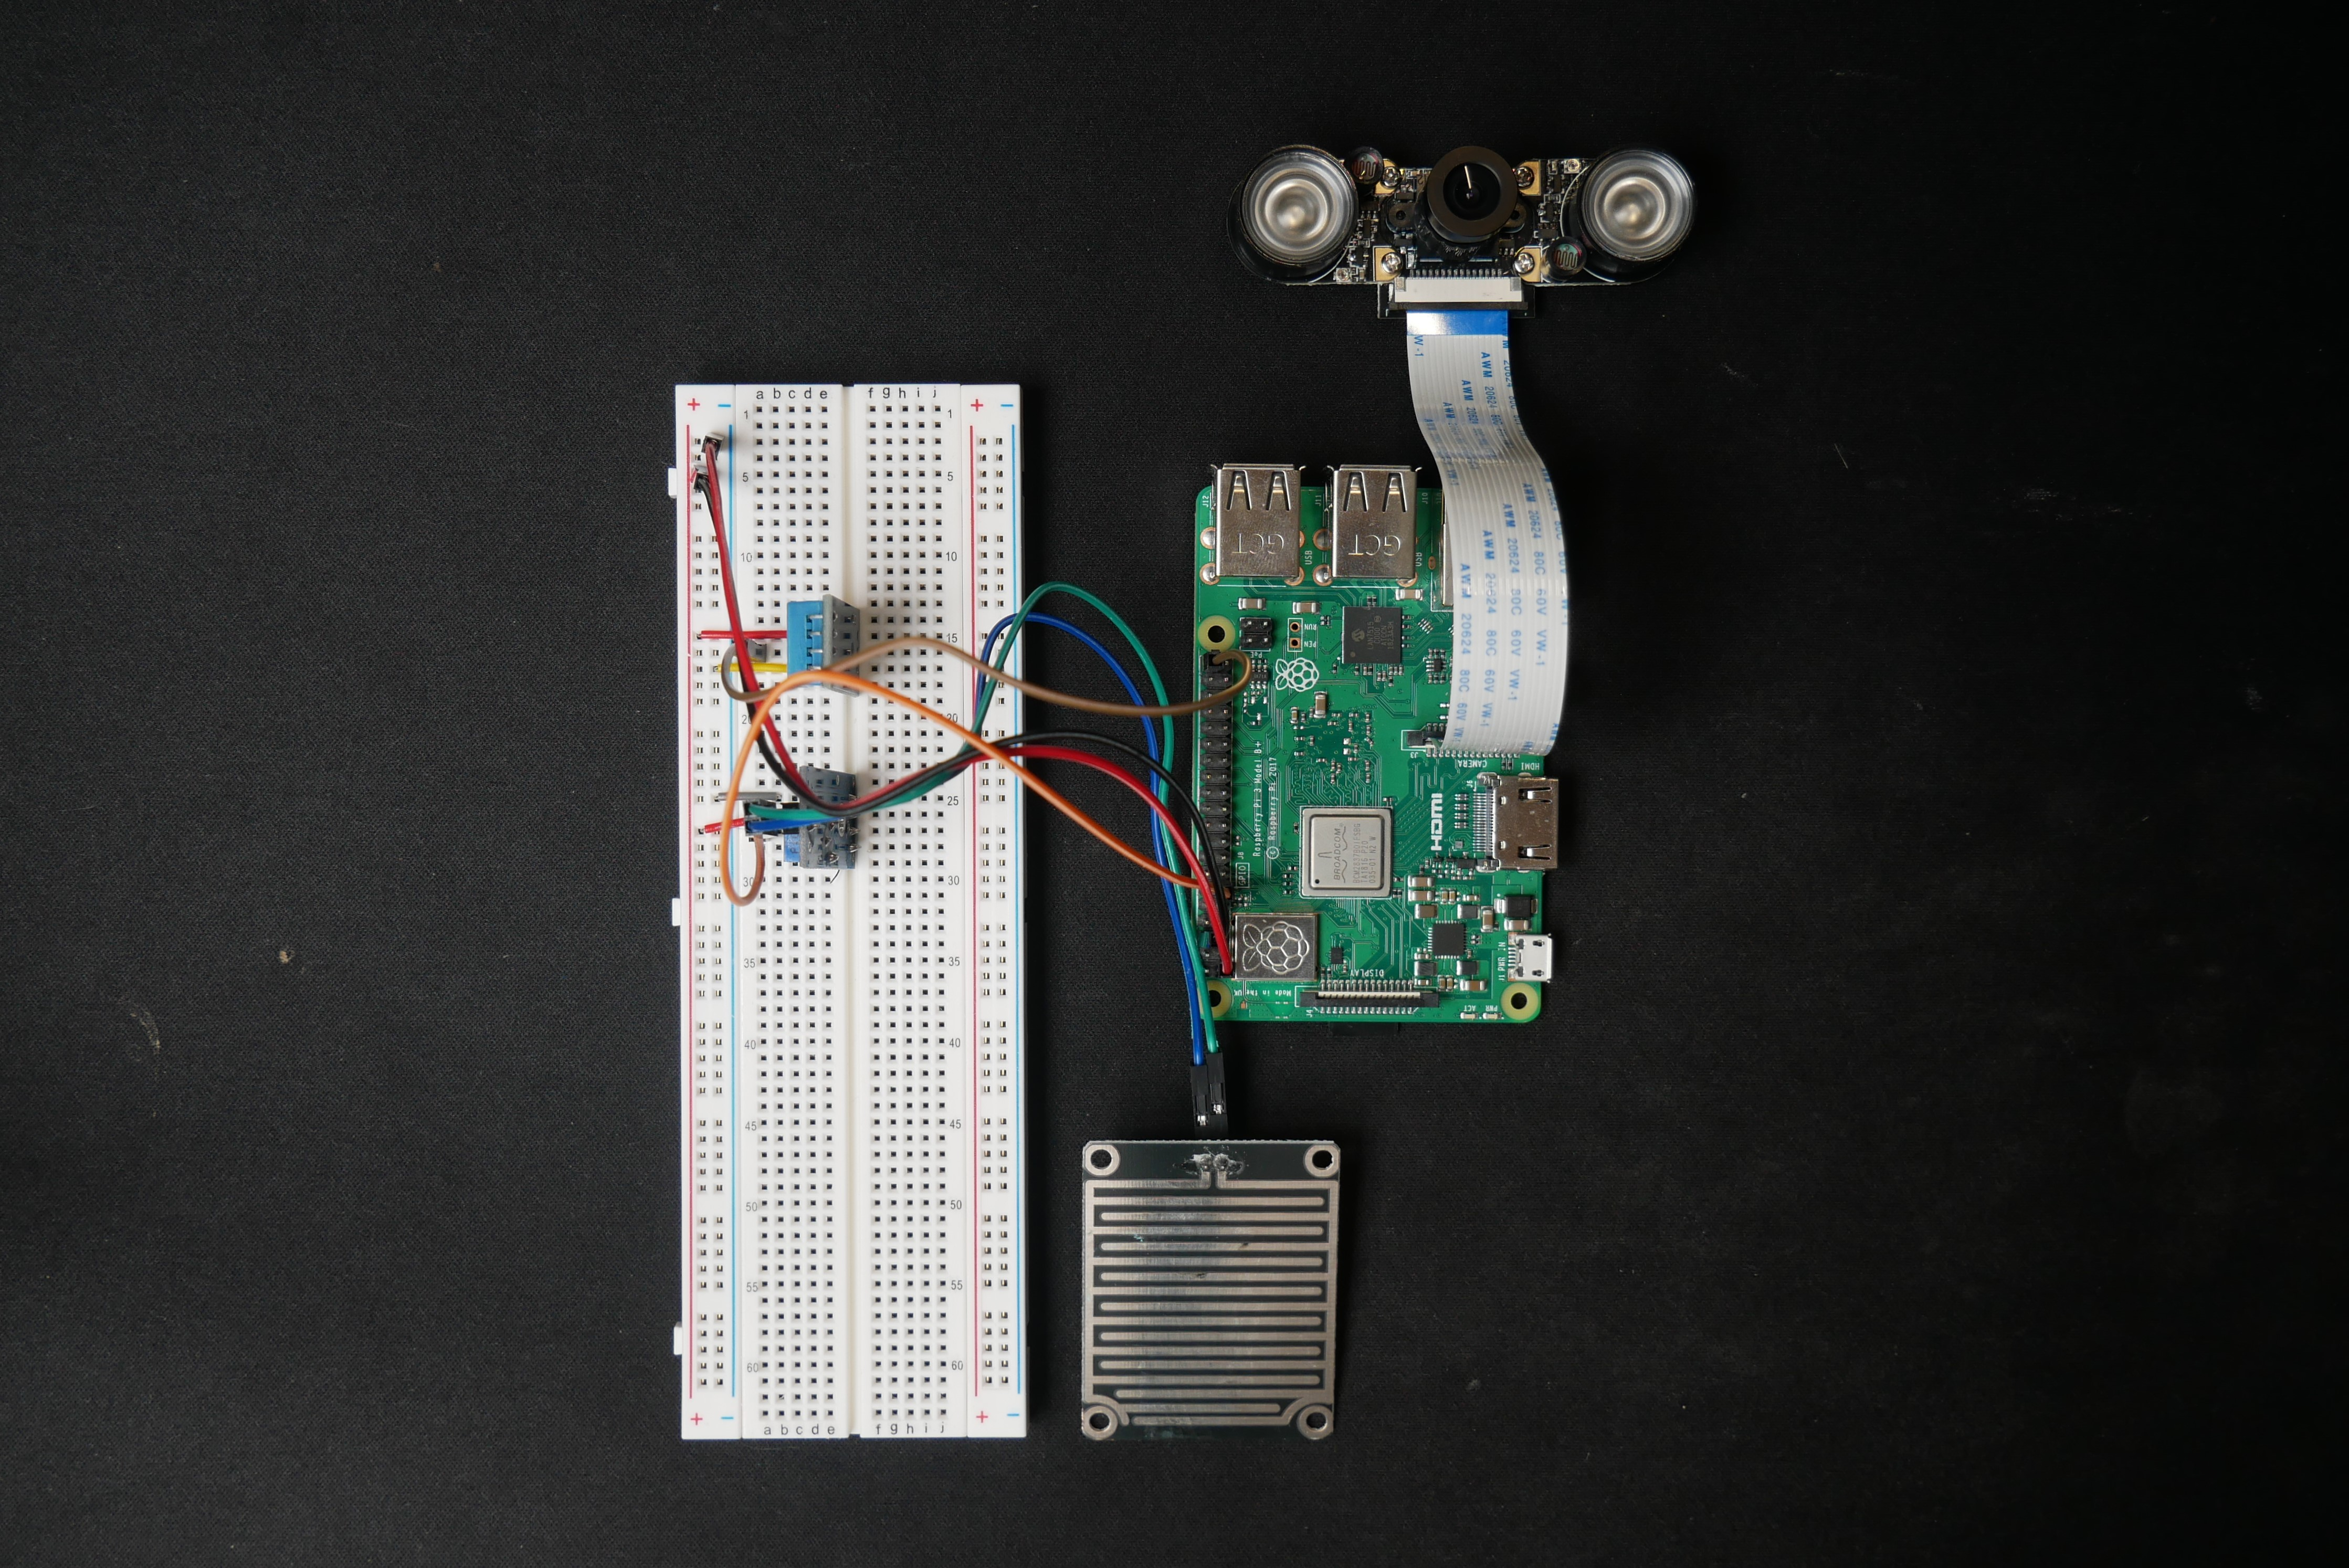
\includegraphics[width=\linewidth]{images/overView.jpg}
    \caption{An overall image of the completed circuit}
    \label{fig:overView}
\end{figure}

INSERT CIRCUIT DIAGRAM

\subsubsection{Circuit Details}
The breadboard is connected to the 3.3v GPIO pin and this supplies power all along the connected rail. There is a 5v pin available however using this requires the inclusion of various resistors in the circuit and this would introduce unnecessary complications. The 3.3v pin also supplies plenty of power for all of the components. A ground pin on the Raspberry Pi is connected to the negative rail on the breadboard. A diagram of the Raspberry Pi Model 3 GPIO pins is shown below. 
\begin{figure}[H]
  \centering
    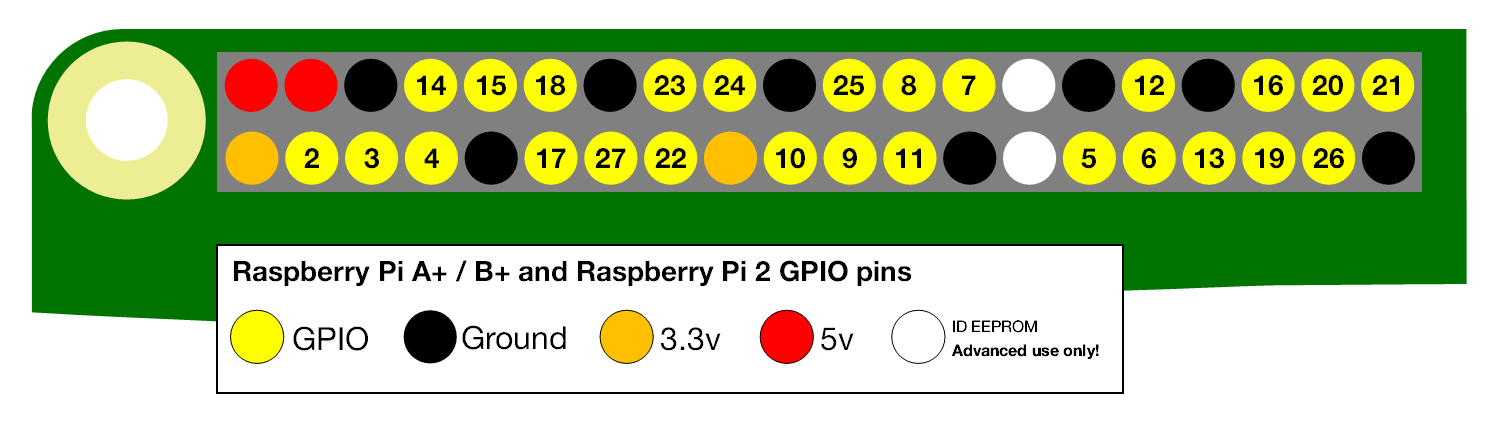
\includegraphics[width=\linewidth]{images/gpio-pins.png}
    \caption{A diagram of the GPIO pins on a Raspberry Pi Model 3}
    \label{fig:gpiopins}
\end{figure}

\begin{figure}[H]
  \centering
    \includegraphics[width=\linewidth]{images/pinCloseUp.jpg}
    \caption{An image of the GPIO pins}
    \label{fig:pinCloseUp}
\end{figure}

Both the FC-37 and DHT11 sensors need 3 of their pins to be connected to the GPIO pins. The FC-37 consists of two components. These are the collector board and electrical board and when enough water is collected on the collector board there is a lower output voltage which signifies rainfall. The collector board connects to the electrical board which in turn connects to the Raspberry Pi. One pin on the electrical board is connected to the power rail on the bread board while another pin is connected to the ground rail. The third pin is the data pin and this is connected to the GPIO pin on the Raspberry Pi. In this case the FC-37 was connected to GPIO pin 27. The electrical board also houses a potentiometer and this can be used to adjust the sensitivity of the collector board. This was done by putting an amount of water onto the collector board and turning the potentiometer until is detected a change in the flow of current.

\begin{figure}[H]
  \centering
    \includegraphics[width=\linewidth]{images/potentiometer.jpg}
    \caption{The small controller board for the rain sensor. This board has a potentiometer which can be used to adjust the sensitivity of the rain sensor.}
    \label{fig:potentiometer}
\end{figure}

\begin{figure}[H]
  \centering
    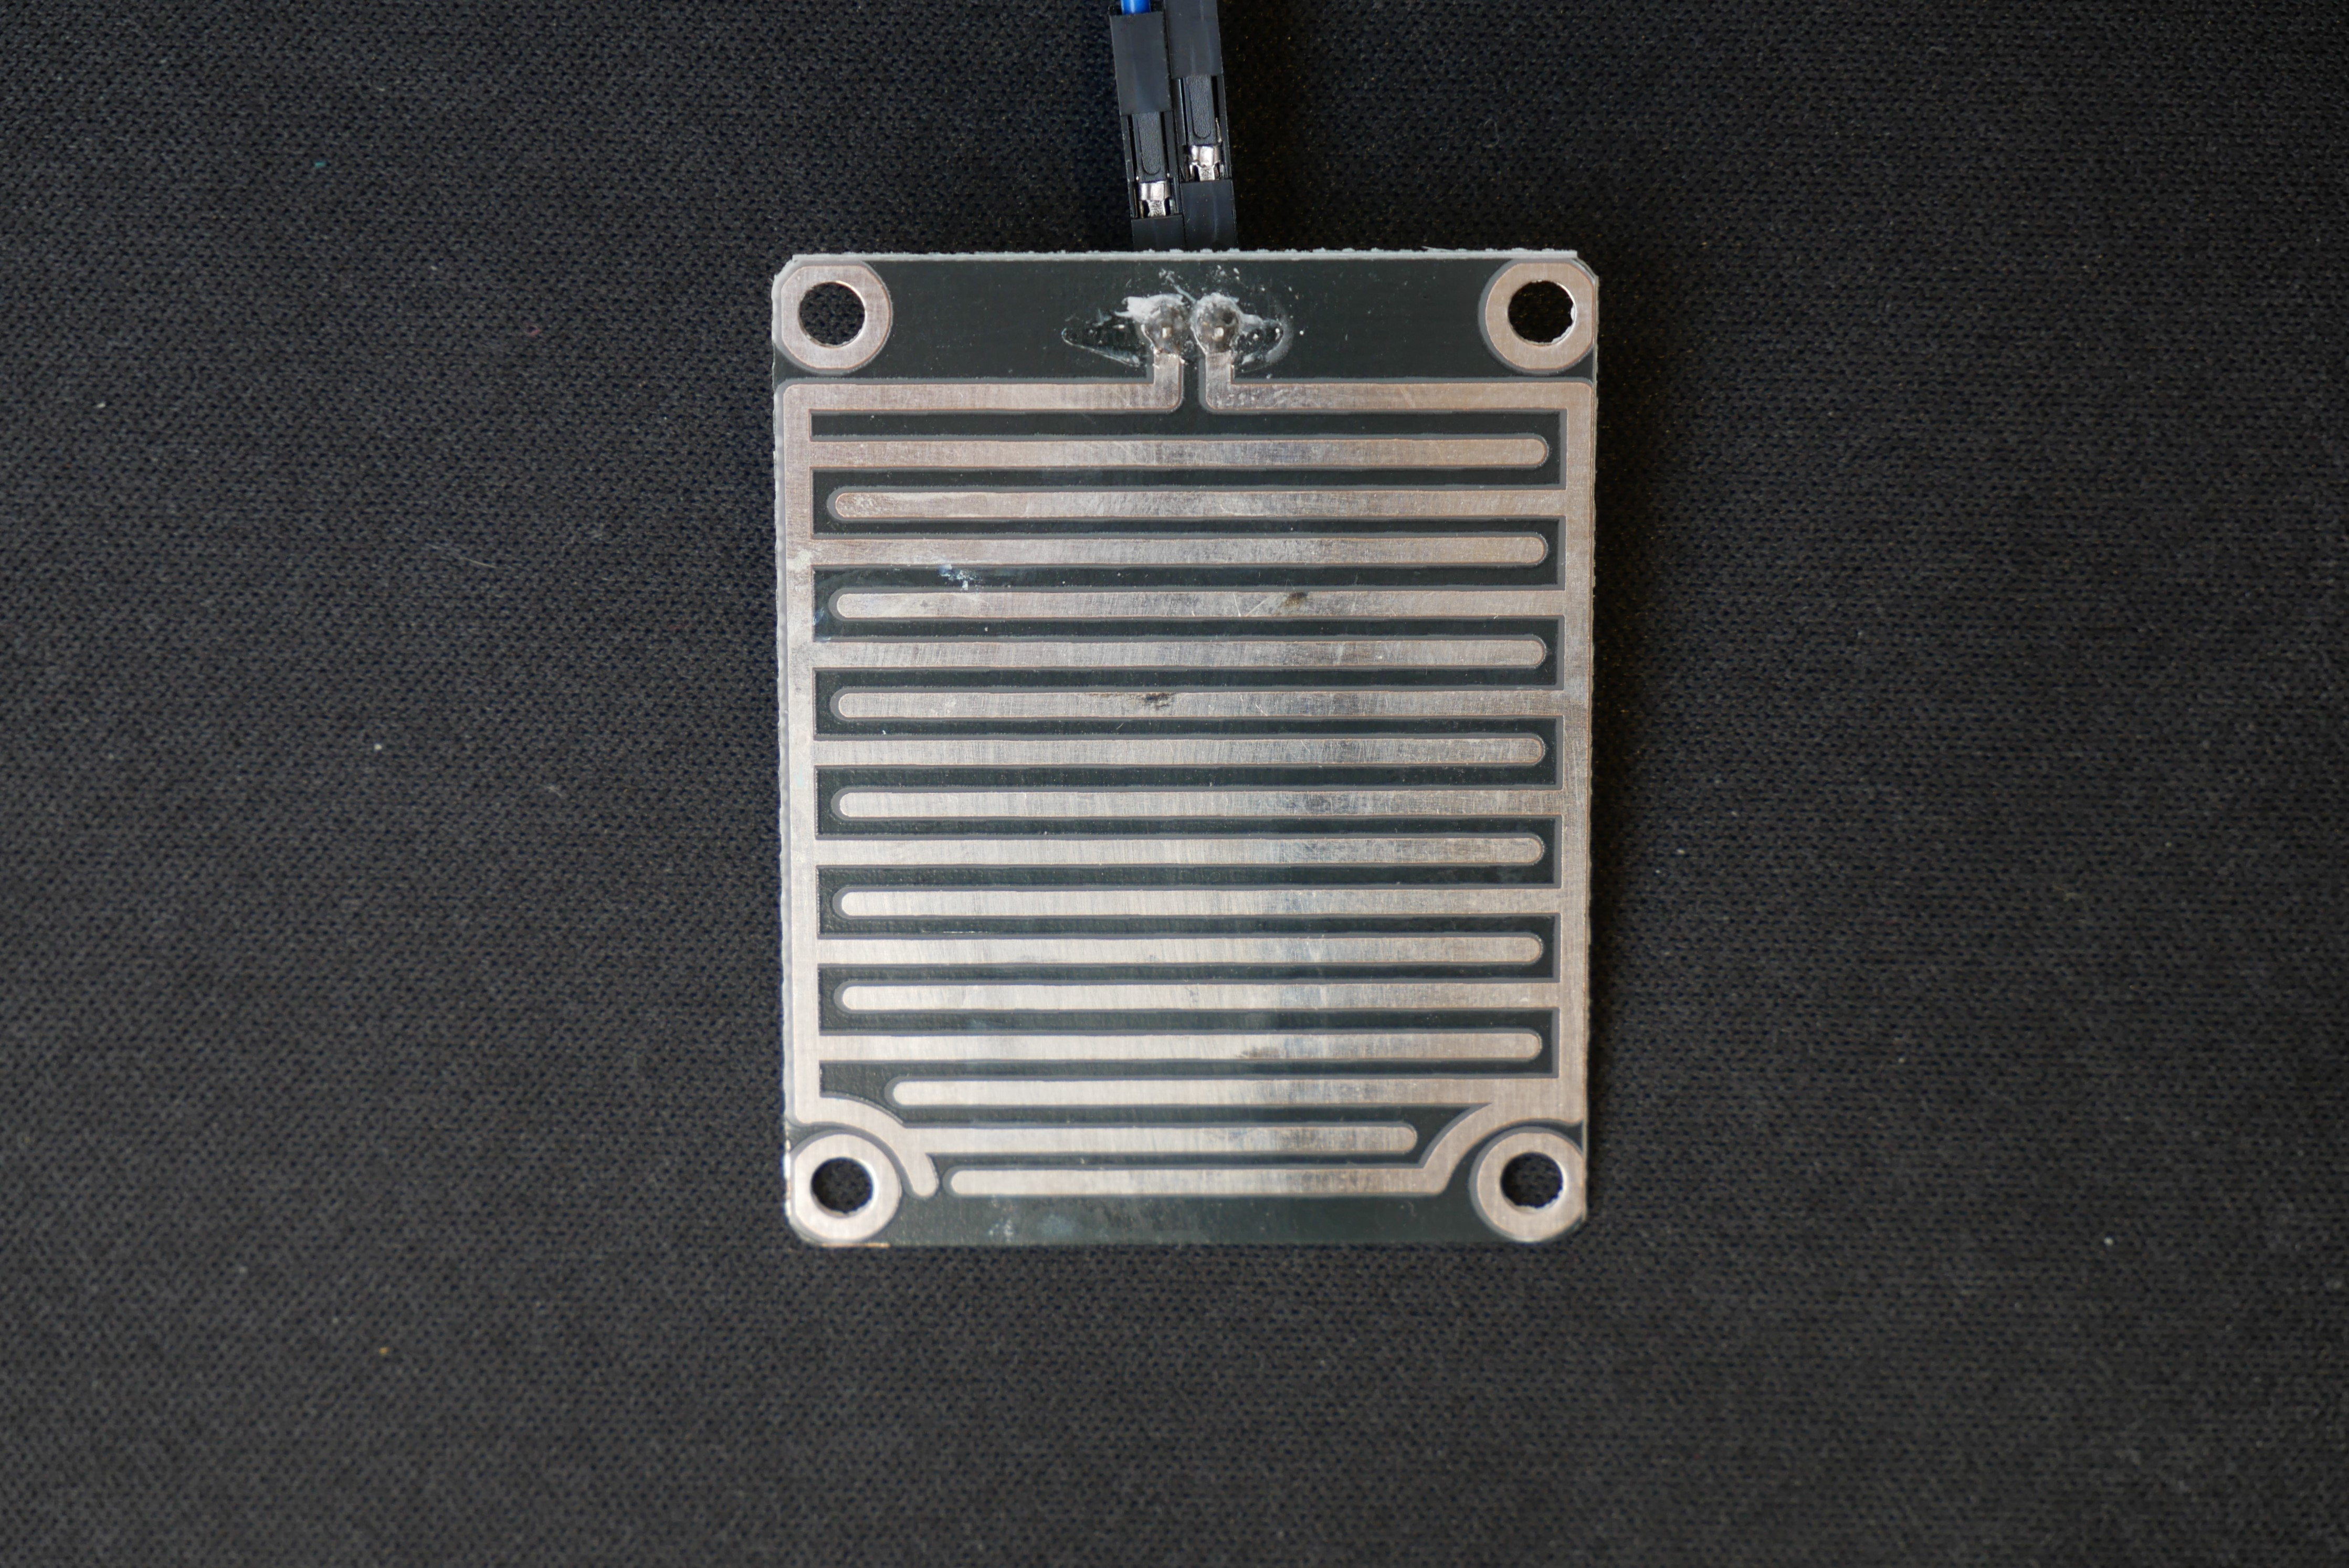
\includegraphics[width=\linewidth]{images/rainPanel.jpg}
    \caption{The FC-37 rain sensor}
    \label{fig:rain panel}
\end{figure}

The DHT11 sensor was connected in a similar way to the FC-37. One sensor pin is connected to the power supply, one to the ground rail and the final pin is connected to a GPIO pin. In this case it was GPIO pin 17. 

\begin{figure}[H]
  \centering
    \includegraphics[width=\linewidth]{images/dht11.jpg}
    \caption{The DHT11 temperature and humidity Sensor.}
    \label{fig:dht11}
\end{figure}

\begin{figure}[H]
  \centering
    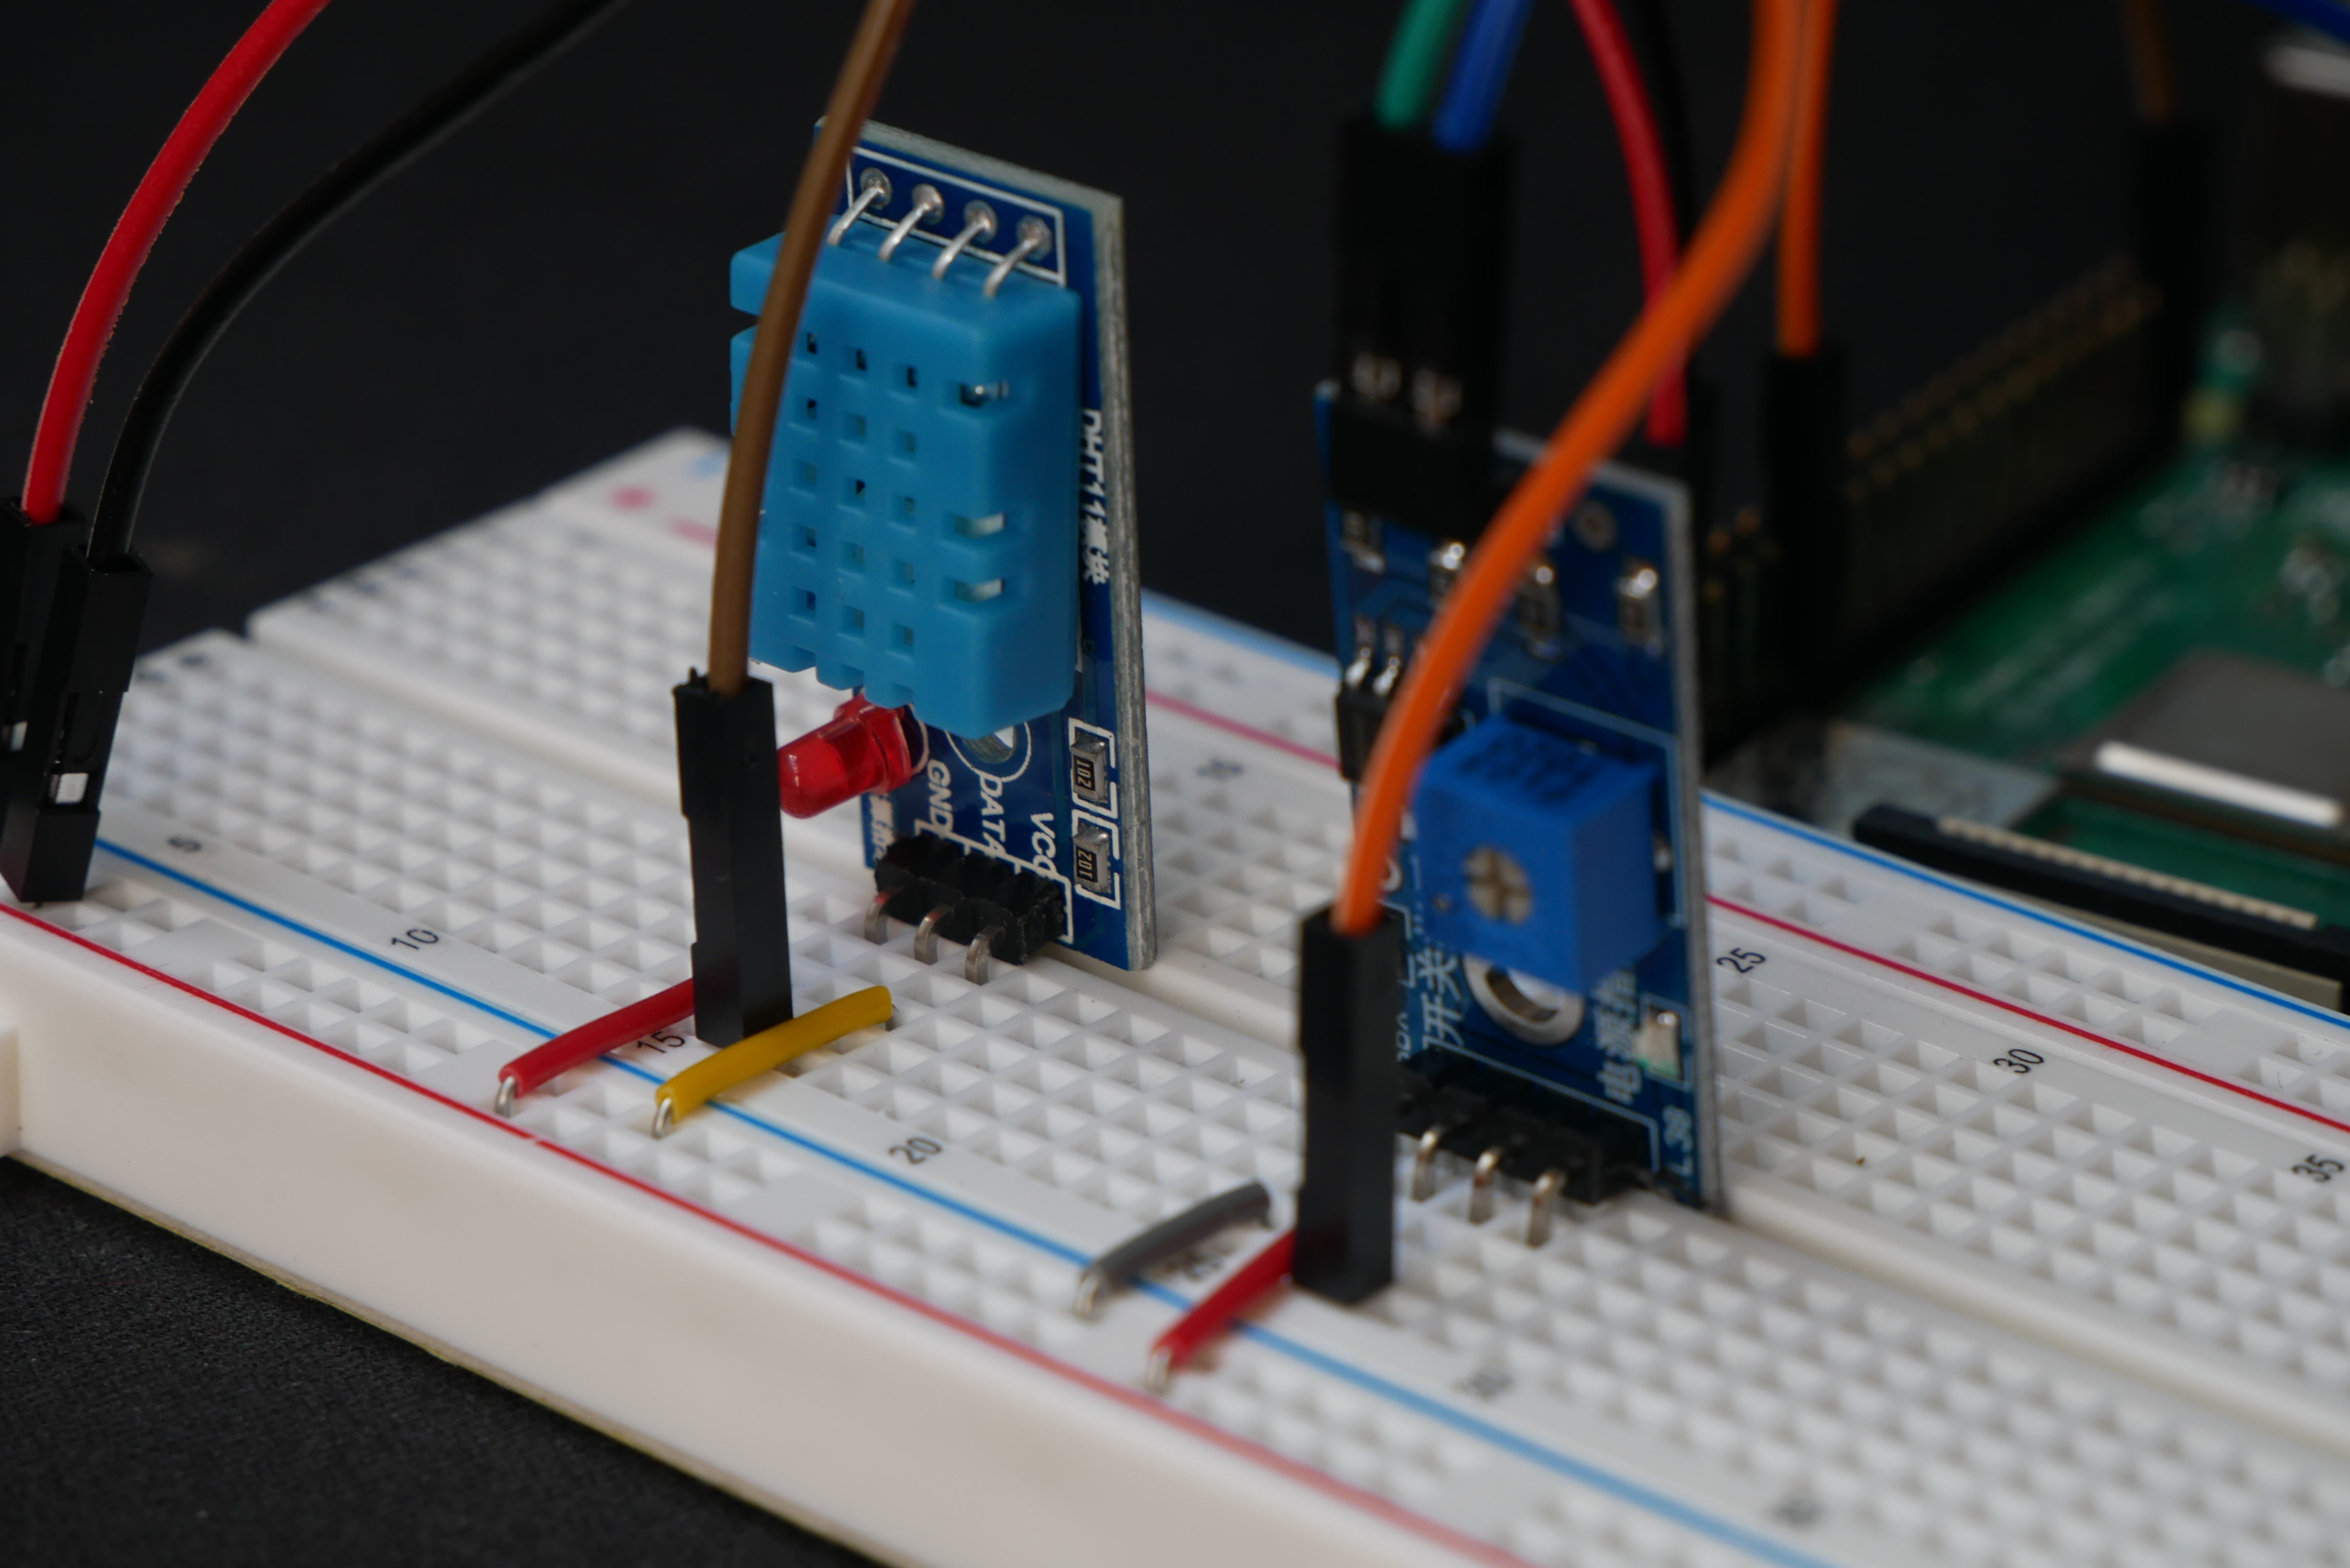
\includegraphics[width=\linewidth]{images/sensorCloseup.jpg}
    \caption{An image showing sensors connected to the breadboard. The DHT11 is on the left and you can see here the three pins on the sensor.}
    \label{fig:piCam}
\end{figure}

The NoIR PiCamera is the least complicated piece of hardware to install. There is already a dedicated slot on the Raspberry Pi which is shown below. The camera is connected into this slot and enabled as described in the previous chapter on the Raspberry Pi itself. 

\begin{figure}[H]
  \centering
    \includegraphics[width=\linewidth]{images/cameraCloseUp.jpg}
    \caption{An image of the slot that the PiCamera goes into}
    \label{fig:piCamCloseUp}
\end{figure}

\subsection{Data Collection}
\subsubsection{dht11.py}
This class was used to collect the temperature and humidity readings from the sensor. I did not write this class. There are many different classes written in Python that will interpret the data from a DHT11 sensor and given that the way the sensor gather data is quite complex, the decision was made to not write this class myself. The DHT11 class is used under the MIT licence - a copy of which can found in the appendixes of this document. 

\subsubsection{rainSensor.py}
This class is what is used to collect rain data. The class contains a constructor function which allows the user to import the class to another Python script. When initialising the new object the user can also use the relevant GPIO pin number as an argument. 

The main function of the class, \texttt{read()}, sets up the GPIO pin. When water is present on the collector board the state of the GPIO will be equal to zero and the function will return \texttt{1} meaning it is raining. Otherwise it will return \texttt{0}. 

\subsubsection{dataSend.py}
This is the main data collection class and ties together the classes outlined above. 

The class has a main function, \texttt{weatherData()}, which collects the data using the classes above and then prints the results to the console. The function then constructs an SQL query and inserts it to the data base. The function is contained within an infinite \texttt{while()} loop and makes use of  \texttt{time.sleep()} so that the amount of time between each dataset can be easily configured. The function is defined at the very beginning of the script. 

The main function is then defined. The first thing this function does is use SSH tunnelling to establish a connection to the database. The database is hosted on PythonAnywhere.com so tunnelling had to be used. I used the \texttt{sshtunnel} Python library to do this. \texttt{MySQL.connector} is then used to establish a connection with the database. The function then checks for a successful connection and if the connection is successful \texttt{weatherData()} will run. Otherwise an error message will be printed to the console. 

An advantage of the above process and the system design is that it isolates the data collection step of the entire process. This way it is very easy to test if the data is being collected and when errors occur they can be quickly diagnosed and resolved. At this point in the process to Raspberry Pi and data collection step is complete. 

\subsection{MySQL Database}
The database is hosted on Python Anywhere and uses MySQL 5.7.21. There are 5 columns in the database and they are listed below. 
\begin{itemize}
\item id - This is just a standard incrementing id field
\item datetime - This stores the datetime value. These values will be used as the labels in the charts
\item temp - holds an int value for the recorded temperature
\item humidity - holds an int value for the recorded humidity percentage. This doesn't need to be a float as the DHT11 sensor will only record humidity in whole integers
\item rain - This is another field with int data type
\end{itemize}

There is the potential for a lot of data to be stored in the data base. The hosting service allows for a size of 1GB which could potentially fill up quite quickly if the project is ever scaled to record more data however currently each row inserted to the database only takes up 84 bytes. In a 1GB database this allows for 12,632,256 rows to be added. If data is sent to the database 18 hours a day every 60 seconds there would be approximately 1080 values being stored each 18 hour period. At this rate it would take 11696 years to fill the database to its 1GB capacity. It is possible to create events in MySQL databases to delete data periodically however in this case it is not necessary. 

\subsection{Data Processing and Presentation}
Now that the data has been recorded and passed from the Raspberry Pi to the database it can be processed and displayed on the web page. Again, Python is being used to achieve this along with other technologies like JSON, Javascript and HTML. Jinja2 template language is available for use within Flask applications however since this is only a single page application it was not needed. 

\subsubsection{Flask\_app.py}
This is the main controller and handles the passing of data to \texttt{main.html}. Navigating to \url{https://www.lukebray.ie/} will return the \texttt{main.html} template. A route has also been set up at \url{https://www.lukebray.ie/get_data/days} to trigger the retrieval and JSON-ification of data from the database. The raw JSON-ified data can be viewed here. Once this route is called a connection to the database is established and a cursor object from \texttt{MySQL.connector} is created. This object is used to execute an SQL query to the database and the requested data is then returned using the \texttt{fetchall()} function and assigned to a variable \texttt{r}. 

The function \texttt{get\_data} performs the initial query to return the most current data values. The function accepts a variable \texttt{days}. This variable is used to determine for how many days the user would like to view historical data. The query to the database is constructed using \texttt{days} and the values are then returned. The nature of this project means that new values are submitted to the database at least every minutes. This is a problem when the user wants to see historical data. For example, one value in the database for every minute over 7 days means returning over 10'000 values which would render a chart virtually useless. To overcome this problem I have used the Pandas\cite{pandas} library which allows the application to take a large amount of data and summarise it. For the 30 day and 7 day periods I have chosen to summarise the data by day but for the 1 day period the data is summarised by hour. For the example of 7 days, Pandas can group the data by day and then return the average data value for that day. This is a particularly useful tool to have as it means that massive amounts of data can be grouped together to make the overall data more readable. One other option that was explored was using algorithms such as the Ramer-Douglas-Peucker\cite{douglaspeucker} algorithm however this was deemed unsuitable as the data representation using Pandas and averages was more accurate. 

Four empty Python lists are instantiated - one for each column in the database excluding the id column. A \texttt{for} loop now runs through all of the returned rows and for each row inserts the relevant piece of data into the relevant list. 

Since the rain sensor returns a value of -1 if it isn't raining I decided to add some extra code here to assign a value of \texttt{True} or \texttt{False} depending on the integer that is in the database. This made it easier going forward to get a quick idea of the value. 

The lists are then converted to a JSON format using the JSON library for Python and stored in an array called \texttt{payload}. The most current data values are also stored here. 

\subsubsection{main.html}
This file is where the data is displayed to the user. Bootstrap and JQuery were used to give the page a nice look and feel. These libraries also help with keeping the page so that it is responsive and will work across many devices. The charts were made using the charts.js library for Javascript. The Javascript logic is contained below the HTML content and I will explain it below. 

After the global variables and chart canvas have been declared a number of functions are created. 
\paragraph{getFreshData()}
This function is used to do the Ajax call which gets the set of data requested. It takes \texttt{days} as an argument and is called from buttons within the HTML. 

Ajax stands for Asynchronous Javascript and XML and it is the Asynchronous nature of the call that I had the biggest issue to overcome. \texttt{getFreshData()} can easily make the Ajax call however it cannot process any of the data that is returned from the call. For example, the application retrieves all of the data in one large array. These need to be split into smaller arrays such as \texttt{\_rainData} and \texttt{\_humData}. Because the call is Asynchronous and Javascript executes sequentially it means that the next lines of Javascript are already executing before the Ajax call can return the data. Because the data is always changing it needs to be retrieved every few seconds. This fact combined with the Asynchronous nature of Ajax calls meant that I could not have a single function to get the data and assign the variables. The solution to this issue will be explained below as it is influenced by another factor of the design. 

\paragraph{createLineChart(chartName, theData, canvas)}
This function takes 3 arguments and is used to actually construct the chart. All of the chart options such as colours and tick options are set in this function and can be called at any time to create a chart. 

\paragraph{initialiseChart(days)}
This is the function that gets the data and draws the chart. It also processes the data which is passed from \texttt{Flask\_app.py}. The function uses \texttt{getFreshData()} to retrieve the data and then assigns various pieces of data to variables that were earlier declared as global. Then the function defines the chart data and uses \texttt{createLineChart()} to draw the chart. 

\paragraph{historicChart()}
This function takes an argument of \texttt{days}. A global boolean variable called \texttt{liveData} has already been set with a default value of \texttt{true}. This function first sets that value to \texttt{false} and then calls \texttt{initialiseChart()} to draw the historic chart. When this function is called a static chart is displayed on the page. The function is called when buttons within the HTML are clicked. For example the 7 day button has an attribute \texttt{onclick="historicData(7)"}. 

\paragraph{liveChart()}
This function is used to draw a live chart which updates every x seconds. The chart will be set to update every 60 seconds. The function calls \texttt{initialiseChart()} and the sets \texttt{liveData = true}. Then every x seconds the function will check to see if \texttt{liveData} is still true. This is so that when a historic chart is called the page won't reload with a live chart - it will display a static historic chart. 

\paragraph{Page Operation}
When the page is loaded an initial chart is drawn. This will be a live chart that is continuously updating since I have set \texttt{liveData = true} by default. There is also some logic that checks for this value and if it is true then \texttt{liveChart()} is called. This allows the user to switch back to a live chart after they have viewed a historic chart. \texttt{liveChart()} is called from the live chart button which sets \texttt{liveData = true} which in turn allows the application to call \texttt{liveChart()}. This is effectively a \texttt{while} loop used to keep the live charts updating continuously. 

The Ajax calls are resolved within \texttt{initialiseChart()}. The call is made using \texttt{getFreshData()}. The returned JSON array is then parsed and split into smaller arrays and variables as follows: 
\begin{itemize}
\item \texttt{\_tempData}
\item \texttt{\_humData}
\item \texttt{\_isRaining}
\item \texttt{\_currentTemp} (variable)
\item \texttt{\_currentHum} (variable)
\item \texttt{\_labels}
\end{itemize}

This is advantageous in that it means the data is current however it does mean that \texttt{flask\_app.py} is making constant calls to the database. Unfortunately due to the nature of this project constant calls are made to the database when a live chart is being viewed. However that is unavoidable given the nature of the project. Fortunately using Javascript with Charts.js means most of the real data processing is done client-side. 

\pagebreak
\section{Testing and Evaluation}
\subsection{Introduction}
There are many steps to ensuring this particular device works properly and the final data results are displayed to the user in the proper way. The project has been designed to be modular and this makes testing a lot easier to conduct. Each component can be tested before being implemented and this has meant that combining all components into the final project has been quick and efficient.

This section will explain the testing methodology and show how each component was tested before being implemented fully. 
Why testing is important for this product and what tests need to be done to ensure a good prototype
\subsection{Testing Methodology}
To ensure a good prototype the testing was to be split into multiple phases. Once the tests in each phase have been passed then development on the next phase can begin.
\subsubsection{PiCamera Testing}
This was the first component to be tested. The criteria for passing the test were as follows: 
\begin{enumerate}
  \item The camera can record an image in the dark
  \item The video can be viewed on Youtube without significant interruption
\end{enumerate}

To satisfy the first requirement a still image was taken in a dark room using the Camera library for Python. This test would confirm that the camera can take a still image and also that the infra-red LED attachments work. Below is the successful test image. 

\begin{figure}[H]
  \centering
    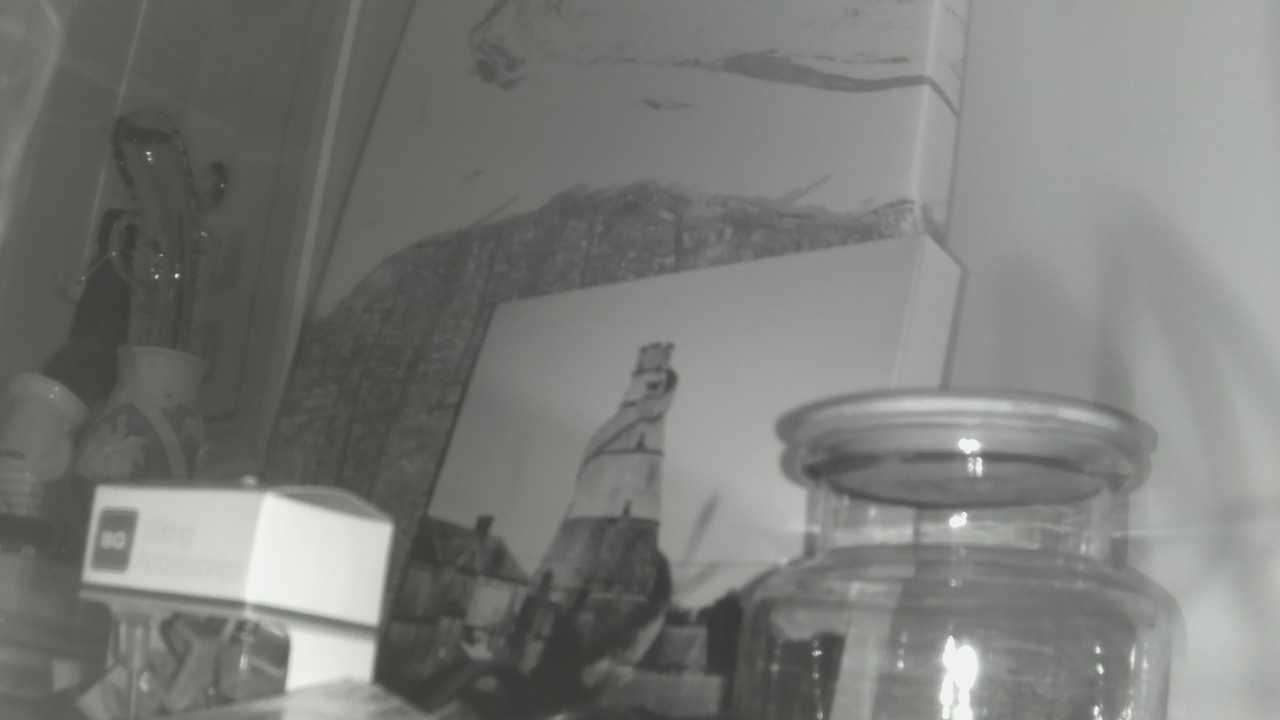
\includegraphics[width=\linewidth]{images/testimage.jpg}
    \caption{A test image taken with the infra-red PiCamera}
    \label{fig:cameraTest}
\end{figure}

The second requirement was satisfied by navigating to the livestream URL and confirming that the camera was streaming video footage. The device was left to run for an hour to ensure it would not go down. This test was passed however there were some minor interruptions in the video streaming. The quality of the video can be lowered so that less data needs to be transmitted. 

\subsubsection{Sensor Testing}
The device receives multiple inputs from the sensors attached and testing the functionality of these was an important step. The requirements of the testing of each sensor was the same and so the same tests could be ran for each sensor. The requirements were as follows:
\begin{enumerate}
  \item The sensor can read values in real time and output them to the console
\end{enumerate}

A small script called \texttt{sensorTest.py} was written that would output a value to the console for each sensor every few seconds. Then each sensor was manipulated to see if it was providing live data. The DHT11 sensor was manipulated by covering it with my hand and seeing if the temperature and humidity values changed whilst the rain sensor had a small amount of water put onto it. The testing of the rain sensor failed at first however it was discovered this was because the sensor was not configured to be sensitive enough. After configuration of the rain sensor all sensors passed the testing. 

\subsubsection{Data Collection Testing}
This stage of testing was the first stage where multiple components of the project were combined into one larger component that made up the data collection aspect of the project. This phase of testing tested the data collection script \texttt{dataSend.py} which performed the actual collection of the data as well as sending the data to the database. The requirements were as follows: 

\begin{enumerate}
  \item The app can establish a connection to the database
  \item Data can be recorded and output to the console
  \item Data can be sent to the database
\end{enumerate}

To meet the requirements above, the database was first cleared of any data. Then \texttt{dataSend.py} was set to collect data every 5 seconds and run for 1 minute. Then the MySQL database was checked to first of all see that all of the data had been recorded and also that the expected 12 rows of data were present. This was confirmed and therefore the test was successful.

\subsubsection{Data Display Testing}
This stage of testing was the most difficult to do and it was the stage that required the most iterations to finally meet the passing requirements. To pass this stage of testing the following requirements had to be met:

\begin{enumerate}
  \item The final web page displays a live, responsive chart section
  \item The final web page displays the most recent temperature and humidity values as well as the current rain status
  \item The final web page allows the user the view historic data in predefined date ranges
\end{enumerate}

The testing for this part of the project was done on the live website. Code was updated on PythonAnywhere and then the website refreshed to evaluate the changes. \texttt{console.log(var)} was used to evaluate that the correct values were being passed from the controller. Using Python Anywhere I was also able to view the error logs and server logs. So if anything went wrong with the front end template I could view it in the web browser console and anything that went wrong with the backend controller could be viewed using the logs on Python Anywhere. 

I also used the web browser to test the web page on different devices to verify its responsiveness. 

\subsection{Evaluation}
Overall the device performed well on most of the tests. The majority of tests were passed within 2 or 3 iterations of the test being run and this indicates that the design was well thought out. The most troublesome testing came during the data display testing and this took many iterations to eventually meet the testing requirements and be suitable for deployment. 

After completing all of the testing and having a working prototype it is useful to see if the initial design requirements have been met.
\begin{table}[]
  \begin{tabular}{@{}cc@{}}
  \toprule
  \multicolumn{1}{l}{\textbf{Requirement Reference}} & \multicolumn{1}{l}{\textbf{Requirement Met?}} \\ \midrule
  SR001                                              & Yes                                           \\
  SR002                                              & Yes                                           \\
  SR003                                              & Yes                                           \\
  SR004                                              & Yes                                           \\
  SR005                                              & No                                            \\
  SR006                                              & No                                            \\
  SR007                                              & Yes                                           \\
  SR008                                              & Yes                                           \\
  SR009                                              & Yes                                           \\
  SR010                                              & Yes                                           \\ \bottomrule
  \end{tabular}
  \caption{System requirements and if they were fulfileld or not}
\label{tab:systemRequirements}
\end{table}

\subsubsection{PiBB - SR001}
\begin{center}
\textit{The system will be able to output a live HD video feed of the inside of the dark nest box. This allows a user to see if anything is living inside of the nest box.}
\linebreak
\end{center}
This requirement has been satisfied by using an infra-red camera and streaming the footage to YouTube. 

\subsubsection{PiBB - SR002}
\begin{center}
\textit{The system will be able to record environmental data about the nest box and send it to a web server.}
\linebreak
\end{center}
This requirement has been satisfied by using the Raspberry Pi and hardware sensors to record the data. \texttt{dataSend.py} has been used to process the data and send it to the web server which is hosted on Python Anywhere. 

\subsubsection{PiBB - SR003}
\begin{center}
\textit{The web server must be able to display live data and the web page must update dynamically to display the latest data}
\linebreak
\end{center}
This requirement has been achieved by using Javascript and Python to retrieve data from the web server and display it on the web page. Using Charts.js has allowed me to create charts that update dynamically.

\subsubsection{PiBB - SR004}
\begin{center}
\textit{The system will be able to interpret the data received from the sensors and display live data on a dynamic web page. This allows a user to see environmental data.}
\linebreak
\end{center}
The data is processed using Python scripts written as controllers using the Flask framework. This framework provided an easy way to process that data and ensure that live data can be passed to the front end template. Using Javascript technologies like Bootstrap and Charts.js allow the web page to be dynamic and let the user view environmental data in a way that is easy to interpret. 

\subsubsection{PiBB - SR005}
\begin{center}
\textit{The system will be able to be deployed remotely and outside. This will mean having a renewable power source and wireless internet connection. The system must be weatherproof.}
\linebreak
\end{center}
This requirement has not been fully achieved. The system has a wireless internet connection and is mostly weatherproof however the power supply is not renewable. During development of the project I discovered that a Raspberry Pi is not suited to being used with a power supply that could be inconsistent (such as solar power would be in Ireland) and so a renewable power source was not used. Having inconsistent power would jeopardise the fulfillment of the other requirements in this project. Another renewable energy source, such as wind, could be used but this would be in a future iteration of the project. 

\subsubsection{PiBB - SR006}
\begin{center}
\textit{The system will be able to manage power failures in a way that does not corrupt or damage files on the system}
\linebreak
\end{center}
This requirement was not met because it is less relevant with the exclusion of renewable energy from the project. Mains power will supply the device and so power failures are less likely. However in a future iteration where a source of renewable energy is used for power this requirement will be a lot more critical and could be a very interesting project by itself.


\subsubsection{PiBB - SR007}
\begin{center}
\textit{The system must not be obtrusive to the wildlife occupying the nest box and must be as discreet as possible. }
\linebreak
\end{center}
This requirement has been met. The system is very small and does not require much interaction once it is up and running. It attaches to the back of the nesting box and so is minimally intrusive to wildlife. 

\subsubsection{PiBB - SR008}
\begin{center}
\textit{It must be possible to access the system remotely to perform necessary software maintenance once it is deployed. }
\linebreak
\end{center}
This requirement has been met and it is possible to access the device remotely as long as power is available. Access is gained through VNC however this does have a drawback in that the remote device and device accessing the remote device must be on the same local network. This can be resolved by setting up port forwarding on the router which the device is connected to however this is beyond the scope of this project. 

\subsubsection{PiBB - SR009}
\begin{center}
\textit{The sensor and camera controllers must be built using Python programming language.}
\linebreak
\end{center} 
This requirement was met. Using Python was a good design element as it is a robust language that is well suited to data processing. 

\subsubsection{PiBB - SR010}
\begin{center}
\textit{The web application should be built using a Python framework.}q
\linebreak
\end{center}
This requirement was achieved by using the Flask framework. Although this project only has one web page using Flask will make it very easy to scale the website in case that is ever required. 

\subsection{Implementation of the Prototype}
The prototype will be implemented in an environment that is not too remote but allows further testing of the functionality of the device in both a software and hardware sense. A garden would be a good place to implement the prototype. The device still needs to be connected to mains power which means it cannot be fully remotely deployed. The weather sealing of the device is still somewhat unknown and adverse weather may affect the device. One potential issue is that the device can get quite hot. To weather seal it the device is placed inside a plastic box and during the summer months airflow may be an issue so the device may overheat. 

Some bugs still remain with the software. The script that controls the DHT11 sensor produces intermittent errors and the cause of these errors is unknown. This will have to be monitored and considered when implementing the prototype. There is also a known but with Charts.js where hovering over the chart can sometimes display historic data so this will need to be considered when deploying the live website. Another charting library may need to be used in a future iteration. 

\pagebreak
\section{Further Work}
How might the device be improved? What extra features could be included next time and how might a different SDLC have an effect on the design and functionality of this product

\pagebreak
\section{Conclusions}
What did I learn while doing this project. What went wrong and what was done well. Is the device created as useful as was initially thought? Is the way I did this project the most effective way to achieve the intended result? 

\pagebreak

\appendix
\section{Application Code}
\subsection{dht11.py}
\begin{minted}[linenos,tabsize=2,breaklines]{python}
    import time
  import RPi


  class DHT11Result:
      'DHT11 sensor result returned by DHT11.read() method'

      ERR_NO_ERROR = 0
      ERR_MISSING_DATA = 1
      ERR_CRC = 2

      error_code = ERR_NO_ERROR
      temperature = -1
      humidity = -1

      def __init__(self, error_code, temperature, humidity):
          self.error_code = error_code
          self.temperature = temperature
          self.humidity = humidity

      def is_valid(self):
          return self.error_code == DHT11Result.ERR_NO_ERROR


  class DHT11:
      'DHT11 sensor reader class for Raspberry'

      __pin = 0

      def __init__(self, pin):
          self.__pin = pin

      def read(self):
          RPi.GPIO.setup(self.__pin, RPi.GPIO.OUT)

          # send initial high
          self.__send_and_sleep(RPi.GPIO.HIGH, 0.05)

          # pull down to low
          self.__send_and_sleep(RPi.GPIO.LOW, 0.02)

          # change to input using pull up
          RPi.GPIO.setup(self.__pin, RPi.GPIO.IN, RPi.GPIO.PUD_UP)

          # collect data into an array
          data = self.__collect_input()

          # parse lengths of all data pull up periods
          pull_up_lengths = self.__parse_data_pull_up_lengths(data)

          # if bit count mismatch, return error (4 byte data + 1 byte checksum)
          if len(pull_up_lengths) != 40:
              return DHT11Result(DHT11Result.ERR_MISSING_DATA, 0, 0)

          # calculate bits from lengths of the pull up periods
          bits = self.__calculate_bits(pull_up_lengths)

          # we have the bits, calculate bytes
          the_bytes = self.__bits_to_bytes(bits)

          # calculate checksum and check
          checksum = self.__calculate_checksum(the_bytes)
          if the_bytes[4] != checksum:
              return DHT11Result(DHT11Result.ERR_CRC, 0, 0)

          # ok, we have valid data, return it
          return DHT11Result(DHT11Result.ERR_NO_ERROR, the_bytes[2], the_bytes[0])

      def __send_and_sleep(self, output, sleep):
          RPi.GPIO.output(self.__pin, output)
          time.sleep(sleep)

      def __collect_input(self):
          # collect the data while unchanged found
          unchanged_count = 0

          # this is used to determine where is the end of the data
          max_unchanged_count = 100

          last = -1
          data = []
          while True:
              current = RPi.GPIO.input(self.__pin)
              data.append(current)
              if last != current:
                  unchanged_count = 0
                  last = current
              else:
                  unchanged_count += 1
                  if unchanged_count > max_unchanged_count:
                      break

          return data

      def __parse_data_pull_up_lengths(self, data):
          STATE_INIT_PULL_DOWN = 1
          STATE_INIT_PULL_UP = 2
          STATE_DATA_FIRST_PULL_DOWN = 3
          STATE_DATA_PULL_UP = 4
          STATE_DATA_PULL_DOWN = 5

          state = STATE_INIT_PULL_DOWN

          lengths = [] # will contain the lengths of data pull up periods
          current_length = 0 # will contain the length of the previous period

          for i in range(len(data)):

              current = data[i]
              current_length += 1

              if state == STATE_INIT_PULL_DOWN:
                  if current == RPi.GPIO.LOW:
                      # ok, we got the initial pull down
                      state = STATE_INIT_PULL_UP
                      continue
                  else:
                      continue
              if state == STATE_INIT_PULL_UP:
                  if current == RPi.GPIO.HIGH:
                      # ok, we got the initial pull up
                      state = STATE_DATA_FIRST_PULL_DOWN
                      continue
                  else:
                      continue
              if state == STATE_DATA_FIRST_PULL_DOWN:
                  if current == RPi.GPIO.LOW:
                      # we have the initial pull down, the next will be the data pull up
                      state = STATE_DATA_PULL_UP
                      continue
                  else:
                      continue
              if state == STATE_DATA_PULL_UP:
                  if current == RPi.GPIO.HIGH:
                      # data pulled up, the length of this pull up will determine whether it is 0 or 1
                      current_length = 0
                      state = STATE_DATA_PULL_DOWN
                      continue
                  else:
                      continue
              if state == STATE_DATA_PULL_DOWN:
                  if current == RPi.GPIO.LOW:
                      # pulled down, we store the length of the previous pull up period
                      lengths.append(current_length)
                      state = STATE_DATA_PULL_UP
                      continue
                  else:
                      continue

          return lengths

      def __calculate_bits(self, pull_up_lengths):
          # find shortest and longest period
          shortest_pull_up = 1000
          longest_pull_up = 0

          for i in range(0, len(pull_up_lengths)):
              length = pull_up_lengths[i]
              if length < shortest_pull_up:
                  shortest_pull_up = length
              if length > longest_pull_up:
                  longest_pull_up = length

          # use the halfway to determine whether the period it is long or short
          halfway = shortest_pull_up + (longest_pull_up - shortest_pull_up) / 2
          bits = []

          for i in range(0, len(pull_up_lengths)):
              bit = False
              if pull_up_lengths[i] > halfway:
                  bit = True
              bits.append(bit)

          return bits

      def __bits_to_bytes(self, bits):
          the_bytes = []
          byte = 0

          for i in range(0, len(bits)):
              byte = byte << 1
              if (bits[i]):
                  byte = byte | 1
              else:
                  byte = byte | 0
              if ((i + 1) % 8 == 0):
                  the_bytes.append(byte)
                  byte = 0

          return the_bytes

      def __calculate_checksum(self, the_bytes):
          return the_bytes[0] + the_bytes[1] + the_bytes[2] + the_bytes[3] & 255
\end{minted}

\subsection{rainSensor.py}
\begin{minted}[linenos,tabsize=2,breaklines]{python}
  import time
  import RPi.GPIO as GPIO

  class RainSensor():
      'Rain sensor reader class'    
      __pin = 0

      #each instance has a self and a gpio pin
      def __init__(self, pin):
          self.__pin = pin
      
      def read(self):
          GPIO.setup(self.__pin, GPIO.IN)
          state = GPIO.input(self.__pin)
          
          if (state == 0):
              return 1
          else:
              return 0
\end{minted}

\subsection{dataSend.py}
\begin{minted}[linenos,tabsize=2,breaklines]{python}
  import RPi.GPIO as GPIO
  import dht11
  import rainSensor
  import time
  import datetime
  import mysql.connector
  from mysql.connector import Error
  import sshtunnel

  GPIO.setwarnings(False)
  GPIO.setmode(GPIO.BCM)
  GPIO.cleanup()

  temphum = dht11.DHT11(pin = 21)
  GPIO.cleanup()

  rain = rainSensor.RainSensor(pin = 17)
  GPIO.cleanup()

  sshtunnel.SSH_TIMEOUT = 5.0
  sshtunnel.TUNNEL_TIMEOUT = 5.0

  def weatherData():
      while True:
              resultDHT = temphum.read()
              resultRain = rain.read()
              if resultDHT.is_valid():
                  print("Last Valid Input: " + str(datetime.datetime.now()))
                  print ("Temperature: %d C" % resultDHT.temperature)
                  print ("Humidity: %d %%" % resultDHT.humidity)
                  print ("Raining?: %d" % resultRain)
                  query = "INSERT INTO data (temp, humidity, rain, datetime) VALUES (%s, %s, %s, %s)"
                  args = (resultDHT.temperature, resultDHT.humidity, resultRain, datetime.datetime.now())

                  cursor.execute(query, args)
                  connection.commit()
                  time.sleep(60)
              else:
                  print("Error ", resultDHT.error_code)


  
  if __name__ == '__main__':
      with sshtunnel.SSHTunnelForwarder(
      ('ssh.pythonanywhere.com'),
      ssh_username='USERNAME', ssh_password='PASSWORD',
      remote_bind_address=('REMOTE_BIND_ADDRESS', 3306)
  ) as tunnel:
          connection = mysql.connector.connect(
          user='USER', password='PASSWORD',
          host='127.0.0.1', port=tunnel.local_bind_port,
          database='DATABASE',       
      )
          db_info = connection.get_server_info()
          if connection.is_connected():
              cursor = connection.cursor()
              print('Connected to MySQL DB...version on ', db_info)
              weatherData()
          else:
              print('Failed to connect to database.')
      
          connection.close()
\end{minted}

\subsection{flask\_app.py}
\begin{minted}[linenos,tabsize=2,breaklines]{python}
  from flask import Flask, render_template, jsonify
  from datetime import datetime, timedelta
  import pandas as pd
  import mysql.connector
  import json

  app = Flask(__name__)

  @app.route('/')
  def index():
      return render_template("main.html")

  @app.route('/get_data/<days>')
  def get_data(days):
      conn = mysql.connector.connect(
      host='HOSTNAME',
      user='USERNAME',
      passwd='PASSWORD',
      db='DATABASE')

      c = conn.cursor()

      days = int(days)

      rows = None

      value = datetime.now() - timedelta(days)
      print(value)

      tempData = []
      humData = []
      rainData = []
      labels = []

      c.execute("SELECT temp, humidity, rain, datetime FROM data ORDER BY datetime DESC LIMIT 1;")
      currentRow = c.fetchall()
      currentData = list(currentRow)

      currentTemp = currentData[0][0]
      currentHum = currentData[0][1]
      currentRain = currentData[0][2]

      if days == 7 or days == 30:
          c.execute("SELECT temp, humidity, rain, datetime FROM data WHERE datetime >= %s ORDER BY datetime DESC;", (value,))

          rows = c.fetchall()

          df = pd.DataFrame(rows, columns=['temp', 'hum', 'rain', 'date']).set_index('date')
          df_day = df.resample('d').mean()
          print('DF_DAY IS BELOW THIS')
          print(df_day)

          for index, row in df_day.iterrows():

              tempData.insert(0, row['temp'])
              humData.insert(0, row['hum'])
              rainData.insert(0, row['rain'])
              labels.insert(0, str(index.date()))

          tempData.reverse()
          humData.reverse()
          rainData.reverse()
          labels.reverse()

          latestRain = rainData[-1]
          isRaining = True

          if (latestRain == 1):
              isRaining = True
          else:
              isRaining = False

          return jsonify({'payload':json.dumps({'tempData':tempData, 'humData':humData, 'isRaining':isRaining, 'labels':labels, 'currentTemp':currentTemp, 'currentHum':currentHum, 'currentRain':currentRain})})

      elif days == 1:
          c.execute("SELECT temp, humidity, rain, datetime FROM data WHERE datetime >= %s ORDER BY datetime DESC;", (value,))

          rows = c.fetchall()

          df = pd.DataFrame(rows, columns=['temp', 'hum', 'rain', 'date']).set_index('date')
          df_hour = df.resample('H').mean()
          print('DF_HOUR IS BELOW THIS')
          print(df_hour)

          for index, row in df_hour.iterrows():

              tempData.insert(0, row['temp'])
              humData.insert(0, row['hum'])
              rainData.insert(0, row['rain'])
              labels.insert(0, str(index.time()))

          tempData.reverse()
          humData.reverse()
          rainData.reverse()
          labels.reverse()

          latestRain = rainData[-1]
          isRaining = True

          if (latestRain == 1):
              isRaining = True
          else:
              isRaining = False

          return jsonify({'payload':json.dumps({'tempData':tempData, 'humData':humData, 'isRaining':isRaining, 'labels':labels, 'currentTemp':currentTemp, 'currentHum':currentHum, 'currentRain':currentRain})})

      else:
          c.execute("SELECT temp, humidity, rain, datetime FROM data ORDER BY datetime DESC LIMIT 25;")
          currentRows = c.fetchall()

          for r in currentRows:

              data = list(r)

              temp = data[0]
              tempData.insert(0, temp)

              hum = data[1]
              humData.insert(0, hum)

              rain = data[2]
              rainData.insert(0, rain)

              datetimeval = str(data[3])
              labels.insert(0, datetimeval)

          latestRain = rainData[-1]
          isRaining = True

          if (latestRain == 1):
              isRaining = True
          else:
              isRaining = False

              return jsonify({'payload':json.dumps({'tempData':tempData, 'humData':humData, 'isRaining':isRaining, 'labels':labels, 'currentTemp':currentTemp, 'currentHum':currentHum, 'currentRain':currentRain})})

  if __name__ == "__main__":
      app.run()
\end{minted}

\subsection{main.html}
\begin{minted}[linenos,tabsize=2,breaklines]{html}
  <!DOCTYPE html>
  <html lang="en">

  <head>
      <meta charset="utf-8">
      <title>My test page</title>
      <meta name="viewport" content="width=device-width, initial-scale=1">
      <link rel="stylesheet" href="https://stackpath.bootstrapcdn.com/bootstrap/4.1.0/
      css/bootstrap.min.css"
      integrity="sha384-9gVQ4dYFwwWSjIDZnLEWnxCjeSWFphJiwGPXr1
      jddIhOegiu1FwO5qRGvFXOdJZ4" crossorigin="anonymous">
      <link rel="shortcut icon" href="{{ url_for('static', filename='favicon.ico') }}">
      <script src="https://code.jquery.com/jquery-3.3.1.slim.min.js" integrity="sha384-q8i/X+965DzO0rT7abK41JStQIAqVgRVzpbzo5
      smXKp4YfRvH+8abtTE1Pi6jizo" crossorigin="anonymous"></script>
      <script src="https://cdnjs.cloudflare.com/ajax/libs/popper.js/
      1.14.0/umd/popper.min.js" integrity="sha384-cs/chFZiN24E4KMATLdqdvsezGxaGsi4hLGOzl
      Xwp5UZB1LY//20VyM2taTB4QvJ" crossorigin="anonymous"></script>
      <script src="https://stackpath.bootstrapcdn.com/bootstrap/
      4.1.0/js/bootstrap.min.js" integrity="sha384-uefMccjFJAIv6A+rW+L4AHf99KvxDjWSu1z9
      VI8SKNVmz4sk7buKt/6v9KI65qnm" crossorigin="anonymous"></script>
      <script src="https://cdn.jsdelivr.net/npm/chart.js@2.8.0/dist
      /Chart.min.js"></script>
      <script src="https://ajax.googleapis.com/ajax/libs/jquery
      /3.2.1/jquery.min.js"></script>
  </head>

  <body>
      <div id="wrapper" class="container">
          <!-- Info will go here -->
          <div class="row">
              <div class="col-12">
                  <h2>Welcome to my birdbox site</h2>
                  <p id="info">
                      Lorem ipsum dolor sit amet, consectetur adipiscing elit, sed
                      do eiusmod tempor incididunt ut labore et dolore magna
                      aliqua. A condimentum vitae sapien pellentesque. Ut consequat
                      semper viverra nam libero justo. Quis auctor elit sed vulputate
                      mi sit amet mauris commodo. Tempor nec feugiat nisl pretium.
                      Justo donec enim diam vulputate ut pharetra. Tortor at auctor
                      urna nunc id cursus. Mauris vitae ultricies leo integer malesuada
                      nunc vel risus. Tristique magna sit amet purus. Dui ut ornare
                      lectus sit amet est placerat. Libero volutpat sed cras ornare
                      arcu. In pellentesque massa placerat duis ultricies.
                  </p>
              </div>
          </div>

          <hr>


          <!-- Cards go here -->
          <div class="card-deck">

              <!-- Current Temp -->
              <div class="card bg-light mb-3 text-center">
                  <div class="card-header">Current Temperature</div>
                  <div class="card-body">
                      <h3 class="card-text" id="currentTemp"></h3>
                  </div>
              </div>

              <!-- Current Humidity -->
              <div class="card bg-light mb-3 text-center">
                  <div class="card-header">Current Humidity</div>
                  <div class="card-body">
                      <h3 class="card-text" id="currentHum"></h3>
                  </div>
              </div>

              <!-- Rain Status -->
              <div class="card bg-light mb-3 text-center">
                  <div class="card-header">Rain Status</div>
                  <div class="card-body">
                      <h3 class="card-text" id="currentRain"></h3>
                  </div>
              </div>
          </div>

          <hr>
          <!-- Charts go here -->
          <div class="row">
              <div id="tempHumChart" class="col-12">
                  <h3>Temperature & Humidity Chart</h3>
                  <!-- bar chart canvas element -->
                  <canvas class="my-4 chartjs-render-monitor" id="myChart" height="150px"></canvas>
                  <div class="row">
                      <div id="dropdown" class="col-4">
                          <div class="btn-group" role="group" aria-label="Basic example">
                              <button id="live" class="btn btn-secondary" type="button" onclick="liveChart()">Live Feed</button>
                              <button id="oneDay" class="btn btn-secondary" type="button" onclick="historicChart(1)">Past Day</button>
                              <button id="sevenDay" class="btn btn-secondary" type="button" onclick="historicChart(7)">Past Week</button>
                              <button id="thirtyDay" class="btn btn-secondary" type="button" onclick="historicChart(30)">Past 30 days</button>
                          </div>
                      </div>
                  </div>
              </div>
          </div>

          <hr>

          <!-- Video content goes here -->
          <div class="row">
              <div class="embed-responsive embed-responsive-16by9">
                  <iframe width="560" height="315" src="https://www.youtube.com/embed/Bey4XXJAqS8"
                  frameborder="0" allow="accelerometer; autoplay; encrypted-media; gyroscope; picture-in-picture"
                  allowfullscreen></iframe>
              </div>
          </div>


      </div>
  </body>

  <script>
  // Global parameters and variables:
  Chart.defaults.global.responsive = true;
  Chart.defaults.global.maintainAspectRatio = true;
  Chart.defaults.global.animation.duration = 0;
  Chart.defaults.global.elements.point.radius = 3;
  Chart.defaults.global.elements.point.hoverRadius = 3;

  var _tempData;
  var _humData;
  var _labels;

  var _currentTemp;
  var _currentHum;
  var _isRaining;

  //assign days var
  var days = 33;

  // get chart canvas
  var ctx = document.getElementById("myChart").getContext("2d");

  //function to get new data
  function getFreshData(days) {
      return $.ajax({
          url: "/get_data/" + days,
          type: "GET",
          data: { vals: '' },
      });
  }



  //a function to create charts
  function createLineChart(chartName, theData, canvas) {
      var chartName = new Chart(canvas, {
          type: 'line',
          data: theData,
          options: {
              title: {
                  display: true,
                  text: chartName
              },
              scales: {
                  xAxes: [{
                      ticks: {
                          autoSkip: true
                      }
                  }],
                  yAxes: [{
                      ticks: {
                          min: -10,
                          max: 100
                      }
                  }]
              }
          }
      });
  }

  //create chart function
  function initialiseChart(days){
      console.log(days);
      getFreshData(days).then(function(data) {
          full_data = JSON.parse(data.payload);
          _tempData = full_data['tempData'];
          _humData = full_data['humData'];
          _isRaining = full_data['currentRain'];
          _labels = full_data['labels'];
          _currentTemp = full_data['currentTemp'];
          document.getElementById("currentTemp").innerHTML = _currentTemp + "&#8451;";
          _currentHum = full_data['currentHum'];
          document.getElementById("currentHum").innerHTML = _currentHum + "&#37;";

          //check for rain
          if (_isRaining == 1) {
              document.getElementById("currentRain").innerHTML = "It\'s raining.";
          } else {
              document.getElementById("currentRain").innerHTML = "It\'s not raining.";
          }

          //define chart data
          var chartData = {
              labels: _labels,
              datasets: [{
                  label: 'Temperature',
                  fill: false,
                  borderColor: 'rgba(255, 0, 0, 1.0)',
                  data: _tempData,
              },{
                  label: 'Humidity',
                  fill: false,
                  borderColor: 'rgba(0, 0, 255, 1.0)',
                  data: _humData,
              }]
          };
          createLineChart("Temperature & Humidity Chart", chartData, ctx);
      });
  }

  var liveData = true;
  console.log("global: " + liveData);

  //function for a historic chart
  function historicChart(days) {
      liveData = false;
      initialiseChart(days);
      console.log(_labels);
  }

  //this function is for the live chart
  function liveChart() {
      initialiseChart(33);
      console.log(liveData);
      liveData = true;
      setInterval(function() {
          if (liveData == true) {
              initialiseChart(33);
          }
      }, 5000);
  }

  //create a chart on loading of the page
  $(document).ready(function() {
      initialiseChart(33);
  });

  //does a live chart
  if (liveData == true) {
      console.log(liveData);
      $(document).ready(function() {
          liveChart();
      });
  }

  </script>
  </html>
\end{minted}

\subsection{camTest.py}
\begin{minted}[linenos,tabsize=2,breaklines]{python}
  from picamera import PiCamera
  from time import sleep

  camera = PiCamera()
  camera.start_preview()
  sleep(5)
  camera.capture('/home/pi/Documents/ProjectFiles/PiBirdBox/tests/testimage.jpg')
  camera.stop_preview()
\end{minted}

\subsection{sensorTest.py}
\begin{minted}[linenos,tabsize=2,breaklines]{python}
  import RPi.GPIO as GPIO
  import dht11
  import rainSensor
  import time
  import datetime

  GPIO.setwarnings(False)
  GPIO.setmode(GPIO.BCM)
  GPIO.cleanup()

  temphum = dht11.DHT11(pin = 21)
  GPIO.cleanup()

  rain = rainSensor.RainSensor(pin = 17)
  GPIO.cleanup()

  def sensorTest():
      while True:
              resultDHT = temphum.read()
              resultRain = rain.read()
              if resultDHT.is_valid():
                  print("Last Valid Input: " + str(datetime.datetime.now()))
                  print ("Temperature: %d C" % resultDHT.temperature)
                  print ("Humidity: %d %%" % resultDHT.humidity)
                  print ("Raining?: %d" % resultRain)

              else:
                  print("Error ", resultDHT.error_code)
              
              time.sleep(5)
                  
  if __name__ == "__main__":
    sensorTest()
\end{minted}

\subsection{pandasTest.py}
\begin{minted}[linenos,tabsize=2,breaklines]{python}
  import pandas as pd
  import datetime

  data = [(21, 55, datetime.datetime(2019, 4, 29, 9, 57, 53)), 
  (22, 55, datetime.datetime(2019, 4, 29, 9, 56, 52)), 
  (26, 47, datetime.datetime(2019, 4, 29, 9, 55, 49)), 
  (22, 54, datetime.datetime(2019, 4, 30, 9, 54, 49)), 
  (20, 54, datetime.datetime(2019, 4, 30, 9, 53, 49)), 
  (19, 65, datetime.datetime(2019, 5, 1, 9, 52, 48)), 
  (18, 53, datetime.datetime(2019, 5, 1, 9, 51, 47)), 
  (21, 58, datetime.datetime(2019, 5, 1, 9, 50, 46))]

  df = pd.DataFrame(data, columns=['temp', 'hum', 'date']).set_index('date')
  df_day = df.resample('d').mean()

  print(df_day)

  tempData = []
  humData = []
  labels = []

  for index, row in df_day.iterrows():
      tempData.insert(0, row['temp'])
      humData.insert(0, row['hum'])
      labels.insert(0, index,)

  tempData.reverse()
  humData.reverse()
  labels.reverse()
  print(tempData)
  print(humData)
  print(labels)
  print(labels[0])
\end{minted}

\pagebreak
\bibliographystyle{unsrt}
\bibliography{biblio}

\end{document}
